% Options for packages loaded elsewhere
% Options for packages loaded elsewhere
\PassOptionsToPackage{unicode}{hyperref}
\PassOptionsToPackage{hyphens}{url}
%
\documentclass[
  10pt,
  ignorenonframetext,
  aspectratio=169,
  spanish,
]{beamer}
\newif\ifbibliography
\usepackage{pgfpages}
\setbeamertemplate{caption}[numbered]
\setbeamertemplate{caption label separator}{: }
\setbeamercolor{caption name}{fg=normal text.fg}
\beamertemplatenavigationsymbolsempty
% remove section numbering
\setbeamertemplate{part page}{
  \centering
  \begin{beamercolorbox}[sep=16pt,center]{part title}
    \usebeamerfont{part title}\insertpart\par
  \end{beamercolorbox}
}
\setbeamertemplate{section page}{
  \centering
  \begin{beamercolorbox}[sep=12pt,center]{section title}
    \usebeamerfont{section title}\insertsection\par
  \end{beamercolorbox}
}
\setbeamertemplate{subsection page}{
  \centering
  \begin{beamercolorbox}[sep=8pt,center]{subsection title}
    \usebeamerfont{subsection title}\insertsubsection\par
  \end{beamercolorbox}
}
% Prevent slide breaks in the middle of a paragraph
\widowpenalties 1 10000
\raggedbottom
\AtBeginPart{
  \frame{\partpage}
}
\AtBeginSection{
  \ifbibliography
  \else
    \frame{\sectionpage}
  \fi
}
\AtBeginSubsection{
  \frame{\subsectionpage}
}
\usepackage{iftex}
\ifPDFTeX
  \usepackage[T1]{fontenc}
  \usepackage[utf8]{inputenc}
  \usepackage{textcomp} % provide euro and other symbols
\else % if luatex or xetex
  \usepackage{unicode-math} % this also loads fontspec
  \defaultfontfeatures{Scale=MatchLowercase}
  \defaultfontfeatures[\rmfamily]{Ligatures=TeX,Scale=1}
\fi
\usepackage{lmodern}

\usetheme[]{Madrid}
\usecolortheme[]{dolphin}
\usefonttheme[]{professionalfonts}
\usefonttheme{serif} % use mainfont rather than sansfont for slide text
\ifPDFTeX\else
  % xetex/luatex font selection
  \setmainfont[]{DejaVu Sans}
  \setsansfont[]{DejaVu Sans}
  \setmonofont[]{DejaVu Sans Mono}
\fi
% Use upquote if available, for straight quotes in verbatim environments
\IfFileExists{upquote.sty}{\usepackage{upquote}}{}
\IfFileExists{microtype.sty}{% use microtype if available
  \usepackage[]{microtype}
  \UseMicrotypeSet[protrusion]{basicmath} % disable protrusion for tt fonts
}{}
\makeatletter
\@ifundefined{KOMAClassName}{% if non-KOMA class
  \IfFileExists{parskip.sty}{%
    \usepackage{parskip}
  }{% else
    \setlength{\parindent}{0pt}
    \setlength{\parskip}{6pt plus 2pt minus 1pt}}
}{% if KOMA class
  \KOMAoptions{parskip=half}}
\makeatother

\usepackage{color}
\usepackage{fancyvrb}
\newcommand{\VerbBar}{|}
\newcommand{\VERB}{\Verb[commandchars=\\\{\}]}
\DefineVerbatimEnvironment{Highlighting}{Verbatim}{commandchars=\\\{\}}
% Add ',fontsize=\small' for more characters per line
\usepackage{framed}
\definecolor{shadecolor}{RGB}{241,243,245}
\newenvironment{Shaded}{\begin{snugshade}}{\end{snugshade}}
\newcommand{\AlertTok}[1]{\textcolor[rgb]{0.68,0.00,0.00}{#1}}
\newcommand{\AnnotationTok}[1]{\textcolor[rgb]{0.37,0.37,0.37}{#1}}
\newcommand{\AttributeTok}[1]{\textcolor[rgb]{0.40,0.45,0.13}{#1}}
\newcommand{\BaseNTok}[1]{\textcolor[rgb]{0.68,0.00,0.00}{#1}}
\newcommand{\BuiltInTok}[1]{\textcolor[rgb]{0.00,0.23,0.31}{#1}}
\newcommand{\CharTok}[1]{\textcolor[rgb]{0.13,0.47,0.30}{#1}}
\newcommand{\CommentTok}[1]{\textcolor[rgb]{0.37,0.37,0.37}{#1}}
\newcommand{\CommentVarTok}[1]{\textcolor[rgb]{0.37,0.37,0.37}{\textit{#1}}}
\newcommand{\ConstantTok}[1]{\textcolor[rgb]{0.56,0.35,0.01}{#1}}
\newcommand{\ControlFlowTok}[1]{\textcolor[rgb]{0.00,0.23,0.31}{\textbf{#1}}}
\newcommand{\DataTypeTok}[1]{\textcolor[rgb]{0.68,0.00,0.00}{#1}}
\newcommand{\DecValTok}[1]{\textcolor[rgb]{0.68,0.00,0.00}{#1}}
\newcommand{\DocumentationTok}[1]{\textcolor[rgb]{0.37,0.37,0.37}{\textit{#1}}}
\newcommand{\ErrorTok}[1]{\textcolor[rgb]{0.68,0.00,0.00}{#1}}
\newcommand{\ExtensionTok}[1]{\textcolor[rgb]{0.00,0.23,0.31}{#1}}
\newcommand{\FloatTok}[1]{\textcolor[rgb]{0.68,0.00,0.00}{#1}}
\newcommand{\FunctionTok}[1]{\textcolor[rgb]{0.28,0.35,0.67}{#1}}
\newcommand{\ImportTok}[1]{\textcolor[rgb]{0.00,0.46,0.62}{#1}}
\newcommand{\InformationTok}[1]{\textcolor[rgb]{0.37,0.37,0.37}{#1}}
\newcommand{\KeywordTok}[1]{\textcolor[rgb]{0.00,0.23,0.31}{\textbf{#1}}}
\newcommand{\NormalTok}[1]{\textcolor[rgb]{0.00,0.23,0.31}{#1}}
\newcommand{\OperatorTok}[1]{\textcolor[rgb]{0.37,0.37,0.37}{#1}}
\newcommand{\OtherTok}[1]{\textcolor[rgb]{0.00,0.23,0.31}{#1}}
\newcommand{\PreprocessorTok}[1]{\textcolor[rgb]{0.68,0.00,0.00}{#1}}
\newcommand{\RegionMarkerTok}[1]{\textcolor[rgb]{0.00,0.23,0.31}{#1}}
\newcommand{\SpecialCharTok}[1]{\textcolor[rgb]{0.37,0.37,0.37}{#1}}
\newcommand{\SpecialStringTok}[1]{\textcolor[rgb]{0.13,0.47,0.30}{#1}}
\newcommand{\StringTok}[1]{\textcolor[rgb]{0.13,0.47,0.30}{#1}}
\newcommand{\VariableTok}[1]{\textcolor[rgb]{0.07,0.07,0.07}{#1}}
\newcommand{\VerbatimStringTok}[1]{\textcolor[rgb]{0.13,0.47,0.30}{#1}}
\newcommand{\WarningTok}[1]{\textcolor[rgb]{0.37,0.37,0.37}{\textit{#1}}}

\usepackage{longtable,booktabs,array}
\usepackage{calc} % for calculating minipage widths
\usepackage{caption}
% Make caption package work with longtable
\makeatletter
\def\fnum@table{\tablename~\thetable}
\makeatother
\usepackage{graphicx}
\makeatletter
\newsavebox\pandoc@box
\newcommand*\pandocbounded[1]{% scales image to fit in text height/width
  \sbox\pandoc@box{#1}%
  \Gscale@div\@tempa{\textheight}{\dimexpr\ht\pandoc@box+\dp\pandoc@box\relax}%
  \Gscale@div\@tempb{\linewidth}{\wd\pandoc@box}%
  \ifdim\@tempb\p@<\@tempa\p@\let\@tempa\@tempb\fi% select the smaller of both
  \ifdim\@tempa\p@<\p@\scalebox{\@tempa}{\usebox\pandoc@box}%
  \else\usebox{\pandoc@box}%
  \fi%
}
% Set default figure placement to htbp
\def\fps@figure{htbp}
\makeatother


% definitions for citeproc citations
\NewDocumentCommand\citeproctext{}{}
\NewDocumentCommand\citeproc{mm}{%
  \begingroup\def\citeproctext{#2}\cite{#1}\endgroup}
\makeatletter
 % allow citations to break across lines
 \let\@cite@ofmt\@firstofone
 % avoid brackets around text for \cite:
 \def\@biblabel#1{}
 \def\@cite#1#2{{#1\if@tempswa , #2\fi}}
\makeatother
\newlength{\cslhangindent}
\setlength{\cslhangindent}{1.5em}
\newlength{\csllabelwidth}
\setlength{\csllabelwidth}{3em}
\newenvironment{CSLReferences}[2] % #1 hanging-indent, #2 entry-spacing
 {\begin{list}{}{%
  \setlength{\itemindent}{0pt}
  \setlength{\leftmargin}{0pt}
  \setlength{\parsep}{0pt}
  % turn on hanging indent if param 1 is 1
  \ifodd #1
   \setlength{\leftmargin}{\cslhangindent}
   \setlength{\itemindent}{-1\cslhangindent}
  \fi
  % set entry spacing
  \setlength{\itemsep}{#2\baselineskip}}}
 {\end{list}}
\usepackage{calc}
\newcommand{\CSLBlock}[1]{\hfill\break\parbox[t]{\linewidth}{\strut\ignorespaces#1\strut}}
\newcommand{\CSLLeftMargin}[1]{\parbox[t]{\csllabelwidth}{\strut#1\strut}}
\newcommand{\CSLRightInline}[1]{\parbox[t]{\linewidth - \csllabelwidth}{\strut#1\strut}}
\newcommand{\CSLIndent}[1]{\hspace{\cslhangindent}#1}

\ifLuaTeX
\usepackage[bidi=basic]{babel}
\else
\usepackage[bidi=default]{babel}
\fi
\ifPDFTeX
\else
\babelfont{rm}[]{DejaVu Sans}
\fi
% get rid of language-specific shorthands (see #6817):
\let\LanguageShortHands\languageshorthands
\def\languageshorthands#1{}


\setlength{\emergencystretch}{3em} % prevent overfull lines

\providecommand{\tightlist}{%
  \setlength{\itemsep}{0pt}\setlength{\parskip}{0pt}}



 


% Estilo separado del contenido. Compilación comprobada con XeLaTeX.
\definecolor{SYSBAzul}{HTML}{0B3954}
\definecolor{SYSBVerde}{HTML}{168C91}
\definecolor{SYSBTexto}{HTML}{203E50}
\setbeamercolor{structure}{fg=SYSBAzul}
\setbeamercolor{normal text}{fg=SYSBTexto,bg=white}
\setbeamercolor{frametitle}{fg=white,bg=SYSBAzul}
\setbeamercolor{block title}{fg=white,bg=SYSBAzul}
\setbeamercolor{block body}{fg=SYSBTexto,bg=SYSBAzul!4}
\setbeamerfont{frametitle}{size=\large,series=\bfseries}
\setbeamerfont{footline}{size=\tiny}
\setbeamersize{text margin left=6mm,text margin right=6mm}
\setbeamertemplate{navigation symbols}{}
\setbeamertemplate{footline}{\hfill\textcolor{SYSBAzul}{SYSB\quad\insertframenumber/\inserttotalframenumber}\hspace{6mm}\vspace{2mm}}
\setbeameroption{hide notes}
\setlength{\parskip}{2pt}
\setlength{\abovedisplayskip}{5pt}
\setlength{\belowdisplayskip}{5pt}
\hypersetup{pdftitle={Sistemas y Señales Biomédicos},pdfauthor={Pablo Eduardo Caicedo-Rodríguez}}

\makeatletter
\@ifpackageloaded{tcolorbox}{}{\usepackage[skins,breakable]{tcolorbox}}
\@ifpackageloaded{fontawesome5}{}{\usepackage{fontawesome5}}
\definecolor{quarto-callout-color}{HTML}{909090}
\definecolor{quarto-callout-note-color}{HTML}{0758E5}
\definecolor{quarto-callout-important-color}{HTML}{CC1914}
\definecolor{quarto-callout-warning-color}{HTML}{EB9113}
\definecolor{quarto-callout-tip-color}{HTML}{00A047}
\definecolor{quarto-callout-caution-color}{HTML}{FC5300}
\definecolor{quarto-callout-color-frame}{HTML}{acacac}
\definecolor{quarto-callout-note-color-frame}{HTML}{4582ec}
\definecolor{quarto-callout-important-color-frame}{HTML}{d9534f}
\definecolor{quarto-callout-warning-color-frame}{HTML}{f0ad4e}
\definecolor{quarto-callout-tip-color-frame}{HTML}{02b875}
\definecolor{quarto-callout-caution-color-frame}{HTML}{fd7e14}
\makeatother
\makeatletter
\@ifpackageloaded{caption}{}{\usepackage{caption}}
\AtBeginDocument{%
\ifdefined\contentsname
  \renewcommand*\contentsname{Tabla de contenidos}
\else
  \newcommand\contentsname{Tabla de contenidos}
\fi
\ifdefined\listfigurename
  \renewcommand*\listfigurename{Listado de Figuras}
\else
  \newcommand\listfigurename{Listado de Figuras}
\fi
\ifdefined\listtablename
  \renewcommand*\listtablename{Listado de Tablas}
\else
  \newcommand\listtablename{Listado de Tablas}
\fi
\ifdefined\figurename
  \renewcommand*\figurename{Figura}
\else
  \newcommand\figurename{Figura}
\fi
\ifdefined\tablename
  \renewcommand*\tablename{Tabla}
\else
  \newcommand\tablename{Tabla}
\fi
}
\@ifpackageloaded{float}{}{\usepackage{float}}
\floatstyle{ruled}
\@ifundefined{c@chapter}{\newfloat{codelisting}{h}{lop}}{\newfloat{codelisting}{h}{lop}[chapter]}
\floatname{codelisting}{Listado}
\newcommand*\listoflistings{\listof{codelisting}{Listado de Listados}}
\makeatother
\makeatletter
\makeatother
\makeatletter
\@ifpackageloaded{caption}{}{\usepackage{caption}}
\@ifpackageloaded{subcaption}{}{\usepackage{subcaption}}
\makeatother

\usepackage{bookmark}
\IfFileExists{xurl.sty}{\usepackage{xurl}}{} % add URL line breaks if available
\urlstyle{same}
\hypersetup{
  pdftitle={Sistemas y Señales Biomédicos},
  pdfauthor={Pablo Eduardo Caicedo-Rodríguez},
  pdflang={es},
  hidelinks,
  pdfcreator={LaTeX via pandoc}}


\author{}
\date{}

\begin{document}


\begin{frame}{Sistemas y Señales Biomédicos}
\phantomsection\label{d1-001}
\textbf{Semanas 1--5 · Bioseñales y representación}

Ph. D. Pablo Eduardo Caicedo-Rodríguez

Material de clase y estudio · Ingeniería Biomédica

\note{\textbf{Libro guía:} John Semmlow, \emph{Circuits, Signals, and
Systems for Bioengineers}, 3.ª ed., 2018.

§1.1, \textbf{Why Biomedical Engineers Need To Analyze Signals And
Systems} (página 8 del visor PDF); §2.2, \textbf{Time Domain
Measurements} (página 57 del visor PDF); §2.4, \textbf{Time Domain
Analysis} (página 81 del visor PDF); §3.3, \textbf{Time--Frequency
Transformation Of Continuous Signals} (página 118 del visor PDF).

\textbf{Correspondencia:} Síntesis o encuadre que reúne varias
secciones; no corresponde a un único apartado del libro. Lectura
principal: Semmlow (2018), tercera edición. La correspondencia usa la
edición del archivo aportado, que difiere de la segunda edición de 2012
citada en el microcurrículo.

\textbf{Lectura:} use estas secciones como ruta de preparación y
consulta. La bibliografía aparece al final del bloque.}
\end{frame}

\begin{frame}{Cómo estudiar estas cinco semanas}
\phantomsection\label{d1-002}
\note{\textbf{Libro guía:} John Semmlow, \emph{Circuits, Signals, and
Systems for Bioengineers}, 3.ª ed., 2018.

§1.1, \textbf{Why Biomedical Engineers Need To Analyze Signals And
Systems} (página 8 del visor PDF); §2.2, \textbf{Time Domain
Measurements} (página 57 del visor PDF); §2.4, \textbf{Time Domain
Analysis} (página 81 del visor PDF); §3.3, \textbf{Time--Frequency
Transformation Of Continuous Signals} (página 118 del visor PDF).

\textbf{Correspondencia:} Síntesis o encuadre que reúne varias
secciones; no corresponde a un único apartado del libro.

\textbf{Lectura:} use estas secciones como ruta de preparación y
consulta. La bibliografía aparece al final del bloque.}
\end{frame}

\begin{frame}{Una ruta desde el cuerpo hasta el espectro}
\phantomsection\label{d1-003}
Al terminar la semana 5, el estudiante debe poder:

\begin{enumerate}
\tightlist
\item
  distinguir \textbf{fenómeno fisiológico, bioseñal, medición y
  registro};
\item
  representar y transformar señales en tiempo continuo y discreto;
\item
  calcular e interpretar descriptores temporales;
\item
  segmentar, normalizar y detectar eventos sin perder el significado
  biomédico;
\item
  explicar por qué una señal periódica admite una representación de
  Fourier;
\item
  interpretar espectros de magnitud y fase.
\end{enumerate}

\begin{block}{Idea conductora}

Una bioseñal no es solo una secuencia de números: es una
\textbf{medición imperfecta de un fenómeno fisiológico}, obtenida
mediante una cadena física y analizada para responder una pregunta.

\end{block}

\note{\textbf{Libro guía:} John Semmlow, \emph{Circuits, Signals, and
Systems for Bioengineers}, 3.ª ed., 2018.

§1.1, \textbf{Why Biomedical Engineers Need To Analyze Signals And
Systems} (página 8 del visor PDF); §2.2, \textbf{Time Domain
Measurements} (página 57 del visor PDF); §2.4, \textbf{Time Domain
Analysis} (página 81 del visor PDF); §3.3, \textbf{Time--Frequency
Transformation Of Continuous Signals} (página 118 del visor PDF).

\textbf{Correspondencia:} Síntesis o encuadre que reúne varias
secciones; no corresponde a un único apartado del libro.

\textbf{Lectura:} use estas secciones como ruta de preparación y
consulta. La bibliografía aparece al final del bloque.}
\end{frame}

\begin{frame}{Mapa de las diez sesiones}
\phantomsection\label{d1-004}
\begin{longtable}[]{@{}
  >{\raggedright\arraybackslash}p{(\linewidth - 4\tabcolsep) * \real{0.3333}}
  >{\raggedright\arraybackslash}p{(\linewidth - 4\tabcolsep) * \real{0.3333}}
  >{\raggedright\arraybackslash}p{(\linewidth - 4\tabcolsep) * \real{0.3333}}@{}}
\toprule\noalign{}
\begin{minipage}[b]{\linewidth}\raggedright
Semana
\end{minipage} & \begin{minipage}[b]{\linewidth}\raggedright
Sesión 1
\end{minipage} & \begin{minipage}[b]{\linewidth}\raggedright
Sesión 2
\end{minipage} \\
\midrule\noalign{}
\endhead
1 & Señal, sistema y bioseñal & Origen, ruido, interferencia y
artefacto \\
2 & Representación y descriptores & Señal sinusoidal \\
3 & Operaciones con señales & Rasgos y eventos temporales \\
4 & Segmentación y normalización & Del tiempo a la frecuencia \\
5 & Series de Fourier & Transformada de Fourier \\
\bottomrule\noalign{}
\end{longtable}

Cada sesión combina fundamento, lectura fisiológica, desarrollo
matemático, ejemplo computacional y verificación.

\note{\textbf{Libro guía:} John Semmlow, \emph{Circuits, Signals, and
Systems for Bioengineers}, 3.ª ed., 2018.

§1.1, \textbf{Why Biomedical Engineers Need To Analyze Signals And
Systems} (página 8 del visor PDF); §2.2, \textbf{Time Domain
Measurements} (página 57 del visor PDF); §2.4, \textbf{Time Domain
Analysis} (página 81 del visor PDF); §3.3, \textbf{Time--Frequency
Transformation Of Continuous Signals} (página 118 del visor PDF).

\textbf{Correspondencia:} Síntesis o encuadre que reúne varias
secciones; no corresponde a un único apartado del libro.

\textbf{Lectura:} use estas secciones como ruta de preparación y
consulta. La bibliografía aparece al final del bloque.}
\end{frame}

\begin{frame}{Organización de cada sesión y trabajo independiente}
\phantomsection\label{d1-005}
\begin{longtable}[]{@{}llr@{}}
\toprule\noalign{}
Momento & Actividad & Tiempo \\
\midrule\noalign{}
\endhead
Apertura & Lectura previa y predicción & 10 min \\
Fundamento & Ecuación, supuestos y ejemplo & 30 min \\
Aplicación & Cálculo o código en parejas & 30 min \\
Cierre & Comprobación individual y límites & 20 min \\
\bottomrule\noalign{}
\end{longtable}

\begin{block}{Nota}

Prepare la lectura en inglés indicada en las notas. Use las ampliaciones
como consulta y trabajo independiente según los conocimientos previos
del grupo.

\end{block}

\note{\textbf{Libro guía:} John Semmlow, \emph{Circuits, Signals, and
Systems for Bioengineers}, 3.ª ed., 2018.

§1.1.1, \textbf{Goals Of This Book} (página 10 del visor PDF).

\textbf{Correspondencia:} Organización docente basada en las actividades
y RAE del microcurrículo. No corresponde a una sección temática del
libro. Microcurrículo: actividades de aprendizaje y RAE, PDF 2--3.
Distribución docente propuesta para las sesiones de 90 minutos.

\textbf{Lectura:} use estas secciones como ruta de preparación y
consulta. La bibliografía aparece al final del bloque.}
\end{frame}

\begin{frame}{Evidencias de aprendizaje y criterios de revisión}
\phantomsection\label{d1-006}
\begin{longtable}[]{@{}
  >{\raggedright\arraybackslash}p{(\linewidth - 2\tabcolsep) * \real{0.5000}}
  >{\raggedright\arraybackslash}p{(\linewidth - 2\tabcolsep) * \real{0.5000}}@{}}
\toprule\noalign{}
\begin{minipage}[b]{\linewidth}\raggedright
Evidencia
\end{minipage} & \begin{minipage}[b]{\linewidth}\raggedright
Criterio observable
\end{minipage} \\
\midrule\noalign{}
\endhead
Lectura y explicación oral & Identifica el supuesto del texto y lo
explica con sus palabras \\
Cálculo individual & Procedimiento correcto, unidades y caso límite \\
Cuaderno en parejas & Código reproducible, datos trazables y
comprobación numérica \\
Informe breve & Interpreta el resultado, cita las fuentes y declara
limitaciones \\
\bottomrule\noalign{}
\end{longtable}

\begin{block}{Concepto clave}

Cada entrega debe permitir distinguir aportes individuales y trabajo
conjunto. La corrección matemática y la justificación biomédica se
revisan por separado. Los porcentajes de evaluación se rigen por el
programa que confirme el profesor.

\end{block}

\note{\textbf{Libro guía:} John Semmlow, \emph{Circuits, Signals, and
Systems for Bioengineers}, 3.ª ed., 2018.

§1.1.1, \textbf{Goals Of This Book} (página 10 del visor PDF).

\textbf{Correspondencia:} Organización docente basada en las actividades
y RAE del microcurrículo. No corresponde a una sección temática del
libro. Microcurrículo: RAE y actividades de evaluación, PDF 2--3. No se
resuelven aquí las inconsistencias administrativas del documento.

\textbf{Lectura:} use estas secciones como ruta de preparación y
consulta. La bibliografía aparece al final del bloque.}
\end{frame}

\begin{frame}[fragile]{Convenciones de los ejemplos en Python}
\phantomsection\label{d1-007}
Los fragmentos que usan \texttt{x} y \texttt{fs} reciben una señal real,
unidimensional, finita y uniformemente muestreada. En la actividad,
documente unidades y metadatos antes de sustituirla.

\begin{Shaded}
\begin{Highlighting}[]
\ImportTok{import}\NormalTok{ numpy }\ImportTok{as}\NormalTok{ np}
\NormalTok{fs }\OperatorTok{=} \FloatTok{256.0}
\NormalTok{t }\OperatorTok{=}\NormalTok{ np.arange(}\DecValTok{2048}\NormalTok{)}\OperatorTok{/}\NormalTok{fs}
\NormalTok{x }\OperatorTok{=}\NormalTok{ np.cos(}\DecValTok{2}\OperatorTok{*}\NormalTok{np.pi}\OperatorTok{*}\DecValTok{10}\OperatorTok{*}\NormalTok{t) }\OperatorTok{+} \FloatTok{.3}\OperatorTok{*}\NormalTok{np.sin(}\DecValTok{2}\OperatorTok{*}\NormalTok{np.pi}\OperatorTok{*}\DecValTok{23}\OperatorTok{*}\NormalTok{t)}
\NormalTok{L, H, Nfft }\OperatorTok{=} \DecValTok{256}\NormalTok{, }\DecValTok{128}\NormalTok{, }\DecValTok{512}
\end{Highlighting}
\end{Shaded}

\begin{block}{Nota}

Este es un ejemplo sintético en unidades arbitrarias. Las variables
específicas de una actividad (etiquetas, sujetos, umbrales, referencias)
deben definirse para ese problema. Los casos reproducibles están en
\texttt{codigo/ejemplos\_verificados.py}.

\end{block}

\note{\textbf{Libro guía:} John Semmlow, \emph{Circuits, Signals, and
Systems for Bioengineers}, 3.ª ed., 2018.

§1.1.1, \textbf{Goals Of This Book} (página 10 del visor PDF).

\textbf{Correspondencia:} Ejemplo, figura o implementación de
elaboración docente a partir de estos fundamentos. No es una
transcripción del código MATLAB del libro. El lenguaje del
microcurrículo suministrado es Python. El libro guía utiliza MATLAB; se
conservan conceptos y se explicitan diferencias de convenciones.

\textbf{Lectura:} use estas secciones como ruta de preparación y
consulta. La bibliografía aparece al final del bloque.}
\end{frame}

\begin{frame}{Semana 1 · Señales, sistemas y bioseñales}
\phantomsection\label{d1-008}
\note{\textbf{Libro guía:} John Semmlow, \emph{Circuits, Signals, and
Systems for Bioengineers}, 3.ª ed., 2018.

§1.1, \textbf{Why Biomedical Engineers Need To Analyze Signals And
Systems} (página 8 del visor PDF); §2.2, \textbf{Time Domain
Measurements} (página 57 del visor PDF); §2.4, \textbf{Time Domain
Analysis} (página 81 del visor PDF); §3.3, \textbf{Time--Frequency
Transformation Of Continuous Signals} (página 118 del visor PDF).

\textbf{Correspondencia:} Síntesis o encuadre que reúne varias
secciones; no corresponde a un único apartado del libro.

\textbf{Lectura:} use estas secciones como ruta de preparación y
consulta. La bibliografía aparece al final del bloque.}
\end{frame}

\begin{frame}{Sesión 1 · La pregunta clínica define qué información
importa}
\phantomsection\label{d1-009}
Una medición solo adquiere sentido cuando se vincula con una pregunta:

\begin{itemize}
\tightlist
\item
  \textbf{ECG:} ¿cómo se propaga la activación eléctrica cardíaca?
\item
  \textbf{EMG:} ¿cuándo y con qué patrón se activa un músculo?
\item
  \textbf{EEG:} ¿cómo cambia la actividad eléctrica cortical?
\item
  \textbf{Respiración:} ¿qué ritmo, amplitud o irregularidad presenta el
  ciclo ventilatorio?
\end{itemize}

\begin{alertblock}{No confundir}

El ECG no es ``el corazón'' ni representa directamente la fuerza de
contracción. Registra diferencias de potencial asociadas con la
actividad eléctrica cardíaca, observadas desde una configuración de
electrodos.

\end{alertblock}

\note{\textbf{Libro guía:} John Semmlow, \emph{Circuits, Signals, and
Systems for Bioengineers}, 3.ª ed., 2018.

§1.1, \textbf{Why Biomedical Engineers Need To Analyze Signals And
Systems} (página 8 del visor PDF); §1.2.2, \textbf{Biotransducers And
Common Physiological Measurements} (página 12 del visor PDF).

\textbf{Correspondencia:} El tema se desarrolla en las secciones
indicadas. La redacción es una síntesis docente.

\textbf{Microcurrículo:} semana 1, sesión 1 (sesión global 1). Los
numerales del cronograma son identificadores curriculares; no son los
apartados del libro citados arriba.}
\end{frame}

\begin{frame}{Señal: una variable que porta información}
\phantomsection\label{d1-010}
Una señal puede representarse como una función:

\[x: \mathcal{D}\rightarrow\mathcal{C},\qquad x(t)\ \text{o}\ x[n]\]

\begin{itemize}
\tightlist
\item
  \(\mathcal{D}\): dominio de la variable independiente, usualmente
  tiempo.
\item
  \(\mathcal{C}\): conjunto de valores de amplitud.
\item
  \(x(t)\): señal en tiempo continuo.
\item
  \(x[n]\): secuencia indexada en tiempo discreto.
\end{itemize}

\begin{block}{Concepto clave}

La señal es una \textbf{representación}. La información fisiológica útil
depende del fenómeno, del sensor, de la ubicación, del protocolo y del
objetivo del análisis.

\end{block}

\note{\textbf{Libro guía:} John Semmlow, \emph{Circuits, Signals, and
Systems for Bioengineers}, 3.ª ed., 2018.

§1.2.3, \textbf{Signal Representation: Continuous (Analog) Signals
Versus Discrete (Digital) Signals} (página 14 del visor PDF).

\textbf{Correspondencia:} El tema se desarrolla en las secciones
indicadas. La redacción es una síntesis docente.

\textbf{Microcurrículo:} semana 1, sesión 1 (sesión global 1). Los
numerales del cronograma son identificadores curriculares; no son los
apartados del libro citados arriba.}
\end{frame}

\begin{frame}{Sistema: una transformación con propósito}
\phantomsection\label{d1-011}
Un sistema relaciona una entrada y una salida:

\[y=\mathcal{T}\{x\}\]

Ejemplos biomédicos:

\begin{itemize}
\tightlist
\item
  sistema cardiovascular: control y demanda \(\rightarrow\) presión y
  flujo;
\item
  amplificador: señal pequeña \(\rightarrow\) señal medible;
\item
  filtro: registro ruidoso \(\rightarrow\) componentes atenuadas;
\item
  detector: ECG \(\rightarrow\) instantes R.
\end{itemize}

\begin{block}{Concepto clave}

Un sistema puede ser biológico, físico, computacional o híbrido.

\end{block}

\note{\textbf{Libro guía:} John Semmlow, \emph{Circuits, Signals, and
Systems for Bioengineers}, 3.ª ed., 2018.

§1.4, \textbf{Biological Systems} (página 34 del visor PDF); §1.4.5,
\textbf{Biosystems Modeling} (página 46 del visor PDF).

\textbf{Correspondencia:} El tema se desarrolla en las secciones
indicadas. La redacción es una síntesis docente.

\textbf{Microcurrículo:} semana 1, sesión 1 (sesión global 1). Los
numerales del cronograma son identificadores curriculares; no son los
apartados del libro citados arriba.}
\end{frame}

\begin{frame}{Modelo entrada--sistema--salida}
\phantomsection\label{d1-012}
\[\text{estímulo }x(t)\quad\longrightarrow\quad
\boxed{\text{sistema fisiológico }\mathcal{T}}
\quad\longrightarrow\quad\text{respuesta }y(t)\]

\textbf{Ejemplo:} reflejo pupilar.

\begin{itemize}
\tightlist
\item
  Entrada: intensidad luminosa.
\item
  Sistema: retina, vías nerviosas y músculo del iris.
\item
  Salida: diámetro pupilar.
\item
  Perturbaciones: luz ambiental, movimiento, parpadeo y variación
  autónoma.
\end{itemize}

\begin{block}{Nota}

El diagrama es una abstracción. Elegir entradas, salidas y fronteras del
sistema es ya una decisión de modelamiento.

\end{block}

\note{\textbf{Libro guía:} John Semmlow, \emph{Circuits, Signals, and
Systems for Bioengineers}, 3.ª ed., 2018.

§1.4, \textbf{Biological Systems} (página 34 del visor PDF); §1.4.5,
\textbf{Biosystems Modeling} (página 46 del visor PDF).

\textbf{Correspondencia:} El tema se desarrolla en las secciones
indicadas. La redacción es una síntesis docente.

\textbf{Microcurrículo:} semana 1, sesión 1 (sesión global 1). Los
numerales del cronograma son identificadores curriculares; no son los
apartados del libro citados arriba.}
\end{frame}

\begin{frame}{Fuente, estímulo y respuesta}
\phantomsection\label{d1-013}
\begin{longtable}[]{@{}
  >{\raggedright\arraybackslash}p{(\linewidth - 4\tabcolsep) * \real{0.3333}}
  >{\raggedright\arraybackslash}p{(\linewidth - 4\tabcolsep) * \real{0.3333}}
  >{\raggedright\arraybackslash}p{(\linewidth - 4\tabcolsep) * \real{0.3333}}@{}}
\toprule\noalign{}
\begin{minipage}[b]{\linewidth}\raggedright
Concepto
\end{minipage} & \begin{minipage}[b]{\linewidth}\raggedright
Pregunta
\end{minipage} & \begin{minipage}[b]{\linewidth}\raggedright
Ejemplo
\end{minipage} \\
\midrule\noalign{}
\endhead
Fuente & ¿El sistema genera actividad observable sin estímulo explícito?
& Ritmo cardíaco espontáneo \\
Estímulo & ¿Qué señal externa modifica el sistema? & Luz sobre la
retina \\
Respuesta & ¿Qué cambio se observa tras el estímulo? & Constricción
pupilar \\
Perturbación & ¿Qué entrada no controlada altera la salida? & Movimiento
del sujeto \\
\bottomrule\noalign{}
\end{longtable}

\begin{alertblock}{Atención}

La correlación temporal no demuestra causalidad: controle retardos y
confundidores.

\end{alertblock}

\note{\textbf{Libro guía:} John Semmlow, \emph{Circuits, Signals, and
Systems for Bioengineers}, 3.ª ed., 2018.

§1.4, \textbf{Biological Systems} (página 34 del visor PDF); §1.4.5,
\textbf{Biosystems Modeling} (página 46 del visor PDF).

\textbf{Correspondencia:} El tema se desarrolla en las secciones
indicadas. La redacción es una síntesis docente.

\textbf{Microcurrículo:} semana 1, sesión 1 (sesión global 1). Los
numerales del cronograma son identificadores curriculares; no son los
apartados del libro citados arriba.}
\end{frame}

\begin{frame}{Jerarquía de una observación biomédica}
\phantomsection\label{d1-014}
\begin{enumerate}
\tightlist
\item
  \textbf{Fenómeno:} proceso fisiológico real.
\item
  \textbf{Mensurando:} magnitud que se desea medir.
\item
  \textbf{Transducción:} conversión de energía a señal utilizable.
\item
  \textbf{Registro:} valores almacenados con unidades y tiempo.
\item
  \textbf{Rasgo:} descriptor extraído del registro.
\item
  \textbf{Inferencia:} interpretación fisiológica o clínica.
\end{enumerate}

\begin{block}{Concepto clave}

Saltar directamente del registro a la inferencia suele ocultar
supuestos. La trazabilidad exige declarar cada nivel.

\end{block}

\note{\textbf{Libro guía:} John Semmlow, \emph{Circuits, Signals, and
Systems for Bioengineers}, 3.ª ed., 2018.

§1.2.2, \textbf{Biotransducers And Common Physiological Measurements}
(página 12 del visor PDF).

\textbf{Correspondencia:} Ejemplo, figura o implementación de
elaboración docente a partir de estos fundamentos. No es una
transcripción del código MATLAB del libro.

\textbf{Microcurrículo:} semana 1, sesión 1 (sesión global 1). Los
numerales del cronograma son identificadores curriculares; no son los
apartados del libro citados arriba.}
\end{frame}

\begin{frame}{Caso integrador: frecuencia cardíaca desde ECG}
\phantomsection\label{d1-015}
El objetivo no es ``medir frecuencia cardíaca'' de forma directa:

\begin{enumerate}
\tightlist
\item
  electrodos observan diferencias de potencial;
\item
  el acondicionamiento limita y amplifica la señal;
\item
  el registro digital conserva muestras \(x[n]\);
\item
  un detector estima instantes \(t_{R,k}\);
\item
  se calculan intervalos \(RR_k=t_{R,k}-t_{R,k-1}\);
\item
  se estima \(HR_k=60/RR_k\) si \(RR_k\) está en segundos.
\end{enumerate}

\begin{alertblock}{Atención}

Un pico alto no es automáticamente una onda R. Artefactos de movimiento
o estimulación pueden producir máximos espurios.

\end{alertblock}

\note{\textbf{Libro guía:} John Semmlow, \emph{Circuits, Signals, and
Systems for Bioengineers}, 3.ª ed., 2018.

§1.2.2, \textbf{Biotransducers And Common Physiological Measurements}
(página 12 del visor PDF).

\textbf{Correspondencia:} Ejemplo, figura o implementación de
elaboración docente a partir de estos fundamentos. No es una
transcripción del código MATLAB del libro.

\textbf{Microcurrículo:} semana 1, sesión 1 (sesión global 1). Los
numerales del cronograma son identificadores curriculares; no son los
apartados del libro citados arriba.}
\end{frame}

\begin{frame}{Verificación de la sesión 1}
\phantomsection\label{d1-016}
Para un sensor de presión plantar durante la marcha:

\begin{enumerate}
\tightlist
\item
  ¿Cuál es el fenómeno fisiomecánico?
\item
  ¿Cuál es el mensurando?
\item
  ¿Cuál es la variable independiente?
\item
  ¿Qué parte es el sistema?
\item
  ¿Qué inferencia sería razonable y cuál sería excesiva?
\end{enumerate}

\begin{block}{Criterio de logro}

La respuesta debe separar explícitamente cuerpo, sensor, señal
registrada, procesamiento e interpretación.

\end{block}

\note{\textbf{Libro guía:} John Semmlow, \emph{Circuits, Signals, and
Systems for Bioengineers}, 3.ª ed., 2018.

§1.2.1, \textbf{Biological Signal Sources} (página 11 del visor PDF);
§1.2.2, \textbf{Biotransducers And Common Physiological Measurements}
(página 12 del visor PDF).

\textbf{Correspondencia:} Actividad o interpretación biomédica de
elaboración docente apoyada en las secciones indicadas.

\textbf{Microcurrículo:} semana 1, sesión 1 (sesión global 1). Los
numerales del cronograma son identificadores curriculares; no son los
apartados del libro citados arriba.}
\end{frame}

\begin{frame}{Sesión 2 · Las bioseñales expresan distintas formas de
energía}
\phantomsection\label{d1-017}
\begin{longtable}[]{@{}
  >{\raggedright\arraybackslash}p{(\linewidth - 4\tabcolsep) * \real{0.3333}}
  >{\raggedright\arraybackslash}p{(\linewidth - 4\tabcolsep) * \real{0.3333}}
  >{\raggedright\arraybackslash}p{(\linewidth - 4\tabcolsep) * \real{0.3333}}@{}}
\toprule\noalign{}
\begin{minipage}[b]{\linewidth}\raggedright
Origen
\end{minipage} & \begin{minipage}[b]{\linewidth}\raggedright
Variable observable
\end{minipage} & \begin{minipage}[b]{\linewidth}\raggedright
Ejemplos
\end{minipage} \\
\midrule\noalign{}
\endhead
Bioeléctrico & potencial o corriente & ECG, EEG, EMG, EOG \\
Biomecánico & fuerza, presión, desplazamiento & presión arterial,
marcha \\
Bioacústico & presión sonora & fonocardiograma, voz \\
Bioóptico & absorción o reflexión & fotopletismografía, oximetría \\
Bioquímico & concentración o actividad & glucosa, \(\mathrm{pH}\),
gases \\
Térmico & temperatura o radiación & termometría, termografía \\
\bottomrule\noalign{}
\end{longtable}

\begin{block}{Concepto clave}

La modalidad de la bioseñal determina sensores, unidades, ancho de
banda, fuentes de error y límites de interpretación.

\end{block}

\note{\textbf{Libro guía:} John Semmlow, \emph{Circuits, Signals, and
Systems for Bioengineers}, 3.ª ed., 2018.

§1.2.1, \textbf{Biological Signal Sources} (página 11 del visor PDF);
§1.2.2, \textbf{Biotransducers And Common Physiological Measurements}
(página 12 del visor PDF).

\textbf{Correspondencia:} El tema se desarrolla en las secciones
indicadas. La redacción es una síntesis docente.

\textbf{Microcurrículo:} semana 1, sesión 2 (sesión global 2). Los
numerales del cronograma son identificadores curriculares; no son los
apartados del libro citados arriba.}
\end{frame}

\begin{frame}{Del fenómeno al dato: la cadena de observación}
\phantomsection\label{d1-018}
\[\begin{aligned}
\text{fisiología}&\rightarrow\text{energía}\rightarrow\text{sensor}\\
&\rightarrow\text{acondicionamiento}\rightarrow\text{conversión}\\
&\rightarrow\text{datos}\rightarrow\text{decisión}
\end{aligned}\]

Preguntas de control:

\begin{itemize}
\tightlist
\item
  ¿Qué energía llega realmente al sensor?
\item
  ¿Qué parte de la señal altera cada etapa?
\item
  ¿Qué unidades tiene el dato almacenado?
\item
  ¿Qué calibración permite volver a unidades físicas?
\end{itemize}

\begin{block}{Nota}

La adquisición nunca es neutra: introduce sensibilidad, limitación de
banda, ruido, retardo y posible distorsión.

\end{block}

\note{\textbf{Libro guía:} John Semmlow, \emph{Circuits, Signals, and
Systems for Bioengineers}, 3.ª ed., 2018.

§1.2.2, \textbf{Biotransducers And Common Physiological Measurements}
(página 12 del visor PDF); §4.2, \textbf{Data Acquisition And Storage}
(página 175 del visor PDF).

\textbf{Correspondencia:} Ejemplo, figura o implementación de
elaboración docente a partir de estos fundamentos. No es una
transcripción del código MATLAB del libro.

\textbf{Microcurrículo:} semana 1, sesión 2 (sesión global 2). Los
numerales del cronograma son identificadores curriculares; no son los
apartados del libro citados arriba.}
\end{frame}

\begin{frame}{Un modelo aditivo útil, pero incompleto}
\phantomsection\label{d1-019}
\[x_{obs}(t)=s(t)+n(t)+i(t)+a(t)\]

\begin{itemize}
\tightlist
\item
  \(s(t)\): componente fisiológica de interés.
\item
  \(n(t)\): ruido aleatorio del sistema de medición.
\item
  \(i(t)\): interferencia originada por otra fuente.
\item
  \(a(t)\): artefacto asociado con el procedimiento o el sujeto.
\end{itemize}

\begin{alertblock}{Atención}

Este modelo supone suma lineal. En la práctica también existen
saturación, deriva, pérdidas de contacto y acoplamientos no lineales.

\end{alertblock}

\note{\textbf{Libro guía:} John Semmlow, \emph{Circuits, Signals, and
Systems for Bioengineers}, 3.ª ed., 2018.

§1.3.1, \textbf{Biological Noise Sources} (página 26 del visor PDF);
§1.3.2, \textbf{Noise Properties: Additive Gaussian Noise} (página 27
del visor PDF).

\textbf{Correspondencia:} El tema se desarrolla en las secciones
indicadas. La redacción es una síntesis docente.

\textbf{Microcurrículo:} semana 1, sesión 2 (sesión global 2). Los
numerales del cronograma son identificadores curriculares; no son los
apartados del libro citados arriba.}
\end{frame}

\begin{frame}{Ruido, interferencia y artefacto no son sinónimos}
\phantomsection\label{d1-020}
\begin{longtable}[]{@{}
  >{\raggedright\arraybackslash}p{(\linewidth - 4\tabcolsep) * \real{0.3333}}
  >{\raggedright\arraybackslash}p{(\linewidth - 4\tabcolsep) * \real{0.3333}}
  >{\raggedright\arraybackslash}p{(\linewidth - 4\tabcolsep) * \real{0.3333}}@{}}
\toprule\noalign{}
\begin{minipage}[b]{\linewidth}\raggedright
Término
\end{minipage} & \begin{minipage}[b]{\linewidth}\raggedright
Rasgo distintivo
\end{minipage} & \begin{minipage}[b]{\linewidth}\raggedright
Ejemplo
\end{minipage} \\
\midrule\noalign{}
\endhead
Ruido & fluctuación aleatoria no informativa para la tarea & ruido
electrónico térmico \\
Interferencia & señal estructurada de fuente ajena & red eléctrica de
50/60 Hz \\
Artefacto & distorsión ligada a adquisición o conducta & movimiento de
electrodos \\
Variabilidad & cambio fisiológico real & arritmia o modulación
respiratoria \\
\bottomrule\noalign{}
\end{longtable}

\begin{block}{Concepto clave}

Eliminar toda variación ``irregular'' puede destruir información
fisiológica. Primero se clasifica la fuente; después se decide cómo
tratarla.

\end{block}

\note{\textbf{Libro guía:} John Semmlow, \emph{Circuits, Signals, and
Systems for Bioengineers}, 3.ª ed., 2018.

§1.3.1, \textbf{Biological Noise Sources} (página 26 del visor PDF);
§1.3.2, \textbf{Noise Properties: Additive Gaussian Noise} (página 27
del visor PDF).

\textbf{Correspondencia:} El tema se desarrolla en las secciones
indicadas. La redacción es una síntesis docente.

\textbf{Microcurrículo:} semana 1, sesión 2 (sesión global 2). Los
numerales del cronograma son identificadores curriculares; no son los
apartados del libro citados arriba.}
\end{frame}

\begin{frame}{La relación señal--ruido necesita contexto}
\phantomsection\label{d1-021}
Una forma basada en potencia es:

\[\mathrm{SNR}_{dB}=10\log_{10}\left(\frac{P_s}{P_n}\right)\]

Si se comparan amplitudes RMS bajo impedancias equivalentes:

\[\mathrm{SNR}_{dB}=20\log_{10}\left(\frac{x_{s,\mathrm{RMS}}}{x_{n,\mathrm{RMS}}}\right)\]

\begin{alertblock}{Atención}

No puede calcularse una SNR válida si no existe una definición
operacional de ``señal'' y ``ruido'' o una referencia razonable.

\end{alertblock}

\note{\textbf{Libro guía:} John Semmlow, \emph{Circuits, Signals, and
Systems for Bioengineers}, 3.ª ed., 2018.

§1.3.1, \textbf{Biological Noise Sources} (página 26 del visor PDF);
§1.3.2, \textbf{Noise Properties: Additive Gaussian Noise} (página 27
del visor PDF).

\textbf{Correspondencia:} El tema se desarrolla en las secciones
indicadas. La redacción es una síntesis docente.

\textbf{Microcurrículo:} semana 1, sesión 2 (sesión global 2). Los
numerales del cronograma son identificadores curriculares; no son los
apartados del libro citados arriba.}
\end{frame}

\begin{frame}{Artefactos frecuentes por modalidad}
\phantomsection\label{d1-022}
\begin{itemize}
\tightlist
\item
  \textbf{ECG:} movimiento, mal contacto, actividad muscular, deriva de
  línea base.
\item
  \textbf{EMG superficial:} desplazamiento de electrodos, crosstalk,
  cambio de impedancia.
\item
  \textbf{EEG:} parpadeo, movimiento ocular, tensión muscular, cableado.
\item
  \textbf{PPG:} presión del sensor, movimiento, perfusión periférica
  variable.
\item
  \textbf{Respiración:} cambio de postura, habla, tos y desplazamiento
  de banda.
\end{itemize}

\begin{block}{Principio de diseño}

La prevención experimental suele ser mejor que la corrección digital:
fijación, preparación de piel, sincronización y protocolo reducen
errores difíciles de revertir.

\end{block}

\note{\textbf{Libro guía:} John Semmlow, \emph{Circuits, Signals, and
Systems for Bioengineers}, 3.ª ed., 2018.

§1.3.1, \textbf{Biological Noise Sources} (página 26 del visor PDF).

\textbf{Correspondencia:} Actividad o interpretación biomédica de
elaboración docente apoyada en las secciones indicadas.

\textbf{Microcurrículo:} semana 1, sesión 2 (sesión global 2). Los
numerales del cronograma son identificadores curriculares; no son los
apartados del libro citados arriba.}
\end{frame}

\begin{frame}{¿Artefacto o fisiología?}
\phantomsection\label{d1-023}
Evidencias útiles:

\begin{enumerate}
\tightlist
\item
  coherencia con canales auxiliares;
\item
  simultaneidad con una marca de evento;
\item
  morfología y duración plausibles;
\item
  distribución espacial entre sensores;
\item
  respuesta esperada ante un estímulo;
\item
  inspección del montaje o video sincronizado.
\end{enumerate}

\begin{block}{Concepto clave}

La clasificación de un segmento debe sustentarse con evidencia
multimodal o experimental, no solo con su apariencia.

\end{block}

\note{\textbf{Libro guía:} John Semmlow, \emph{Circuits, Signals, and
Systems for Bioengineers}, 3.ª ed., 2018.

§1.3.1, \textbf{Biological Noise Sources} (página 26 del visor PDF).

\textbf{Correspondencia:} Actividad o interpretación biomédica de
elaboración docente apoyada en las secciones indicadas.

\textbf{Microcurrículo:} semana 1, sesión 2 (sesión global 2). Los
numerales del cronograma son identificadores curriculares; no son los
apartados del libro citados arriba.}
\end{frame}

\begin{frame}{Cierre de la semana 1}
\phantomsection\label{d1-024}
\begin{itemize}
\tightlist
\item
  Una señal porta información sobre una variable; un sistema transforma
  señales.
\item
  La bioseñal observada depende del fenómeno y de la cadena de medición.
\item
  Ruido, interferencia, artefacto y variabilidad fisiológica requieren
  tratamientos distintos.
\item
  Toda inferencia debe conservar la trazabilidad desde el mensurando.
\end{itemize}

\begin{block}{Pregunta de salida}

¿Qué error de interpretación aparecería si se tratara una variabilidad
fisiológica real como ``ruido'' y se filtrara agresivamente?

\end{block}

\note{\textbf{Libro guía:} John Semmlow, \emph{Circuits, Signals, and
Systems for Bioengineers}, 3.ª ed., 2018.

§1.2, \textbf{Biosignal: Signals Produced By Living Systems} (página 11
del visor PDF); §1.3, \textbf{Noise} (página 26 del visor PDF).

\textbf{Correspondencia:} Síntesis o encuadre que reúne varias
secciones; no corresponde a un único apartado del libro.

\textbf{Microcurrículo:} semana 1, sesión 2 (sesión global 2). Los
numerales del cronograma son identificadores curriculares; no son los
apartados del libro citados arriba.}
\end{frame}

\begin{frame}{Semana 2 · Representación y descripción temporal}
\phantomsection\label{d1-025}
\note{\textbf{Libro guía:} John Semmlow, \emph{Circuits, Signals, and
Systems for Bioengineers}, 3.ª ed., 2018.

§1.1, \textbf{Why Biomedical Engineers Need To Analyze Signals And
Systems} (página 8 del visor PDF); §2.2, \textbf{Time Domain
Measurements} (página 57 del visor PDF); §2.4, \textbf{Time Domain
Analysis} (página 81 del visor PDF); §3.3, \textbf{Time--Frequency
Transformation Of Continuous Signals} (página 118 del visor PDF).

\textbf{Correspondencia:} Síntesis o encuadre que reúne varias
secciones; no corresponde a un único apartado del libro.

\textbf{Lectura:} use estas secciones como ruta de preparación y
consulta. La bibliografía aparece al final del bloque.}
\end{frame}

\begin{frame}{Sesión 3 · Variable independiente y variable dependiente}
\phantomsection\label{d1-026}
Para una señal temporal:

\[x(t):\ t\mapsto\text{amplitud},\qquad x[n]:\ n\mapsto\text{amplitud}\]

\begin{itemize}
\tightlist
\item
  \(t\) tiene unidades de tiempo.
\item
  \(n\) es un índice entero sin unidades.
\item
  Si el muestreo es uniforme, \(t_n=nT_s=n/f_s\).
\item
  La amplitud conserva las unidades de la magnitud medida o del sistema
  digital.
\end{itemize}

\begin{alertblock}{Atención}

El índice \(n\) no es tiempo físico. Para interpretar duración, retardo
o frecuencia se necesita conocer \(f_s\) o los sellos temporales.

\end{alertblock}

\note{\textbf{Libro guía:} John Semmlow, \emph{Circuits, Signals, and
Systems for Bioengineers}, 3.ª ed., 2018.

§1.2.3, \textbf{Signal Representation: Continuous (Analog) Signals
Versus Discrete (Digital) Signals} (página 14 del visor PDF).

\textbf{Correspondencia:} El tema se desarrolla en las secciones
indicadas. La redacción es una síntesis docente.

\textbf{Microcurrículo:} semana 2, sesión 1 (sesión global 3). Los
numerales del cronograma son identificadores curriculares; no son los
apartados del libro citados arriba.}
\end{frame}

\begin{frame}{Continuo, discreto, analógico y digital}
\phantomsection\label{d1-027}
\begin{longtable}[]{@{}ll@{}}
\toprule\noalign{}
Propiedad & Pregunta \\
\midrule\noalign{}
\endhead
Tiempo continuo & ¿La variable independiente admite cualquier \(t\)? \\
Tiempo discreto & ¿Solo existen valores para índices \(n\)? \\
Amplitud continua & ¿La amplitud admite un continuo de valores? \\
Amplitud cuantizada & ¿La amplitud pertenece a niveles finitos? \\
\bottomrule\noalign{}
\end{longtable}

\begin{block}{Concepto clave}

``Discreto'' describe el eje independiente; ``digital'' suele implicar
además amplitud cuantizada y una codificación numérica.

\end{block}

\note{\textbf{Libro guía:} John Semmlow, \emph{Circuits, Signals, and
Systems for Bioengineers}, 3.ª ed., 2018.

§1.2.3, \textbf{Signal Representation: Continuous (Analog) Signals
Versus Discrete (Digital) Signals} (página 14 del visor PDF).

\textbf{Correspondencia:} El tema se desarrolla en las secciones
indicadas. La redacción es una síntesis docente.

\textbf{Microcurrículo:} semana 2, sesión 1 (sesión global 3). Los
numerales del cronograma son identificadores curriculares; no son los
apartados del libro citados arriba.}
\end{frame}

\begin{frame}{Determinista y aleatoria: una distinción de modelo}
\phantomsection\label{d1-028}
\begin{itemize}
\tightlist
\item
  \textbf{Determinista:} una regla permite especificar cada valor, por
  ejemplo \(x(t)=A\cos(2\pi f_0t+\phi)\).
\item
  \textbf{Aleatoria:} se modela mediante variables aleatorias y
  propiedades estadísticas.
\item
  Una bioseñal registrada es una \textbf{realización} de un proceso
  fisiológico variable.
\end{itemize}

\begin{block}{Nota}

Que una señal sea reproducible parcialmente no la convierte en
determinista. Ritmo, amplitud y morfología cambian intra- e intersujeto.

\end{block}

\note{\textbf{Libro guía:} John Semmlow, \emph{Circuits, Signals, and
Systems for Bioengineers}, 3.ª ed., 2018.

§1.4.1, \textbf{Deterministic Versus Stochastic Signals And Systems}
(página 34 del visor PDF).

\textbf{Correspondencia:} El tema se desarrolla en las secciones
indicadas. La redacción es una síntesis docente.

\textbf{Microcurrículo:} semana 2, sesión 1 (sesión global 3). Los
numerales del cronograma son identificadores curriculares; no son los
apartados del libro citados arriba.}
\end{frame}

\begin{frame}{Media y mediana responden preguntas distintas}
\phantomsection\label{d1-029}
Para \(N\) muestras:

\[\bar{x}=\frac{1}{N}\sum_{n=0}^{N-1}x[n]\]

\begin{itemize}
\tightlist
\item
  La \textbf{media} representa el balance algebraico y es sensible a
  valores extremos.
\item
  La \textbf{mediana} es el percentil 50 y es más robusta a
  observaciones atípicas.
\end{itemize}

\begin{alertblock}{Atención}

En EMG bipolar con oscilación alrededor de cero, una media cercana a
cero no implica ausencia de actividad muscular.

\end{alertblock}

\note{\textbf{Libro guía:} John Semmlow, \emph{Circuits, Signals, and
Systems for Bioengineers}, 3.ª ed., 2018.

§2.2.1, \textbf{Mean And Root Mean Squared Signal Measurements} (página
58 del visor PDF).

\textbf{Correspondencia:} Las secciones aportan el fundamento. La
diapositiva amplía la formulación o precisa condiciones que no se
presentan con idéntica notación en el libro. La media se desarrolla en
§2.2.1; la mediana es un complemento del cronograma.

\textbf{Microcurrículo:} semana 2, sesión 1 (sesión global 3). Los
numerales del cronograma son identificadores curriculares; no son los
apartados del libro citados arriba.}
\end{frame}

\begin{frame}{Varianza y desviación estándar cuantifican dispersión}
\phantomsection\label{d1-030}
Varianza descriptiva del segmento (denominador \(N\)):

\[\sigma_x^2=\frac{1}{N}\sum_{n=0}^{N-1}(x[n]-\bar{x})^2\]

Desviación estándar:

\[\sigma_x=\sqrt{\sigma_x^2}\]

\begin{block}{Comprobación}

La desviación estándar conserva las unidades de \(x\). El estimador
muestral con denominador \(N-1\) tiene otro objetivo; la identidad RMS
de la siguiente diapositiva usa denominador \(N\).

\end{block}

\note{\textbf{Libro guía:} John Semmlow, \emph{Circuits, Signals, and
Systems for Bioengineers}, 3.ª ed., 2018.

§2.2.1, \textbf{Mean And Root Mean Squared Signal Measurements} (página
58 del visor PDF); §2.2.2, \textbf{Variance And Standard Deviation}
(página 64 del visor PDF).

\textbf{Correspondencia:} El tema se desarrolla en las secciones
indicadas. La redacción es una síntesis docente.

\textbf{Microcurrículo:} semana 2, sesión 1 (sesión global 3). Los
numerales del cronograma son identificadores curriculares; no son los
apartados del libro citados arriba.}
\end{frame}

\begin{frame}{Valor RMS: amplitud efectiva}
\phantomsection\label{d1-031}
\[x_{\mathrm{RMS}}=\sqrt{\frac{1}{N}\sum_{n=0}^{N-1}x^2[n]}\]

Relación útil:

\[x_{\mathrm{RMS}}^2=\sigma_x^2+\bar{x}^{2}\]

\begin{itemize}
\tightlist
\item
  Si \(\bar{x}=0\), entonces \(x_{\mathrm{RMS}}=\sigma_x\).
\item
  El RMS no elimina el signo arbitrariamente: mide magnitud cuadrática
  media.
\end{itemize}

\begin{block}{Concepto clave}

En EMG, el RMS de una ventana puede describir nivel de actividad, pero
depende de colocación, ganancia, tejido, ventana y normalización.

\end{block}

\note{\textbf{Libro guía:} John Semmlow, \emph{Circuits, Signals, and
Systems for Bioengineers}, 3.ª ed., 2018.

§2.2.1, \textbf{Mean And Root Mean Squared Signal Measurements} (página
58 del visor PDF); §2.2.2, \textbf{Variance And Standard Deviation}
(página 64 del visor PDF).

\textbf{Correspondencia:} El tema se desarrolla en las secciones
indicadas. La redacción es una síntesis docente.

\textbf{Microcurrículo:} semana 2, sesión 1 (sesión global 3). Los
numerales del cronograma son identificadores curriculares; no son los
apartados del libro citados arriba.}
\end{frame}

\begin{frame}{Energía y potencia media}
\phantomsection\label{d1-032}
Para una secuencia, energía y potencia media se definen como:

\[\begin{aligned}
E_x&=\sum_{n=-\infty}^{\infty}|x[n]|^2,\\
P_x&=\lim_{N\to\infty}\frac{1}{2N+1}\sum_{n=-N}^{N}|x[n]|^2.
\end{aligned}\]

En un registro de \(N\) muestras: \(E_N=\sum_{n=0}^{N-1}|x[n]|^2\) y
\(P_N=E_N/N\).

\begin{alertblock}{Atención}

La integral se aproxima con \(T_s\sum|x[n]|^2\), con unidades
\([x]^2\,\mathrm{s}\). La suma sola tiene unidades \([x]^2\).
Interpretar energía física exige un modelo de conversión.

\end{alertblock}

\note{\textbf{Libro guía:} John Semmlow, \emph{Circuits, Signals, and
Systems for Bioengineers}, 3.ª ed., 2018.

§2.2.1, \textbf{Mean And Root Mean Squared Signal Measurements} (página
58 del visor PDF); §4.3, \textbf{Power Spectrum} (página 191 del visor
PDF).

\textbf{Correspondencia:} Las secciones aportan el fundamento. La
diapositiva amplía la formulación o precisa condiciones que no se
presentan con idéntica notación en el libro.

\textbf{Microcurrículo:} semana 2, sesión 1 (sesión global 3). Los
numerales del cronograma son identificadores curriculares; no son los
apartados del libro citados arriba.}
\end{frame}

\begin{frame}[fragile]{Ejemplo computacional: descriptores explícitos}
\phantomsection\label{d1-033}
\begin{Shaded}
\begin{Highlighting}[]
\ImportTok{import}\NormalTok{ numpy }\ImportTok{as}\NormalTok{ np}

\NormalTok{x }\OperatorTok{=}\NormalTok{ np.asarray(x, dtype}\OperatorTok{=}\BuiltInTok{float}\NormalTok{)}
\NormalTok{media }\OperatorTok{=}\NormalTok{ np.mean(x)}
\NormalTok{mediana }\OperatorTok{=}\NormalTok{ np.median(x)}
\NormalTok{varianza }\OperatorTok{=}\NormalTok{ np.mean((x }\OperatorTok{{-}}\NormalTok{ media)}\OperatorTok{**}\DecValTok{2}\NormalTok{)  }\CommentTok{\# denominador N}
\NormalTok{desv }\OperatorTok{=}\NormalTok{ np.sqrt(varianza)}
\NormalTok{rms }\OperatorTok{=}\NormalTok{ np.sqrt(np.mean(x}\OperatorTok{**}\DecValTok{2}\NormalTok{))}
\NormalTok{energia }\OperatorTok{=}\NormalTok{ np.}\BuiltInTok{sum}\NormalTok{(x}\OperatorTok{**}\DecValTok{2}\NormalTok{)}
\end{Highlighting}
\end{Shaded}

\begin{block}{Nota}

Antes de calcular: comprobar unidades, valores faltantes, saturación,
longitud del segmento y si el segmento es comparable entre sujetos.

\end{block}

\note{\textbf{Libro guía:} John Semmlow, \emph{Circuits, Signals, and
Systems for Bioengineers}, 3.ª ed., 2018.

§2.2.1, \textbf{Mean And Root Mean Squared Signal Measurements} (página
58 del visor PDF); §2.2.2, \textbf{Variance And Standard Deviation}
(página 64 del visor PDF).

\textbf{Correspondencia:} Ejemplo, figura o implementación de
elaboración docente a partir de estos fundamentos. No es una
transcripción del código MATLAB del libro.

\textbf{Microcurrículo:} semana 2, sesión 1 (sesión global 3). Los
numerales del cronograma son identificadores curriculares; no son los
apartados del libro citados arriba.}
\end{frame}

\begin{frame}{Promediado de realizaciones y reducción de ruido}
\phantomsection\label{d1-034}
Si \(x_r[n]=s[n]+v_r[n]\) y los ruidos tienen media cero, varianza
\(\sigma_v^2\) y son incorrelacionados entre realizaciones:

\[\bar x[n]=\frac1R\sum_{r=1}^{R}x_r[n],\qquad
\operatorname{Var}(\bar v[n])=\frac{\sigma_v^2}{R}.\]

\begin{block}{Concepto clave}

El promedio conserva la respuesta repetible y reduce la desviación del
ruido por \(\sqrt R\). Los registros deben estar alineados y
corresponder al mismo estado.

\end{block}

En potenciales evocados, variación de latencia o adaptación puede
ensanchar y atenuar la respuesta promedio.

\note{\textbf{Libro guía:} John Semmlow, \emph{Circuits, Signals, and
Systems for Bioengineers}, 3.ª ed., 2018.

§2.2.3, \textbf{Averaging For Noise Reduction} (página 68 del visor
PDF); §2.2.4, \textbf{Ensemble Averaging} (página 70 del visor PDF).

\textbf{Correspondencia:} El tema se desarrolla en las secciones
indicadas. La redacción es una síntesis docente.

\textbf{Microcurrículo:} semana 2, sesión 1 (sesión global 3). Los
numerales del cronograma son identificadores curriculares; no son los
apartados del libro citados arriba.}
\end{frame}

\begin{frame}{Sesión 4 · La sinusoide como coordenada de oscilación}
\phantomsection\label{d1-035}
\[x(t)=A\cos(2\pi f_0t+\phi)=A\cos(\omega_0t+\phi)\]

\begin{longtable}[]{@{}lll@{}}
\toprule\noalign{}
Parámetro & Significado & Unidad \\
\midrule\noalign{}
\endhead
\(A\) & amplitud pico & unidad de \(x\) \\
\(f_0\) & frecuencia & Hz \\
\(T_0\) & periodo, \(T_0=1/f_0\) & s \\
\(\omega_0\) & frecuencia angular, \(2\pi f_0\) & rad/s \\
\(\phi\) & fase inicial & rad \\
\bottomrule\noalign{}
\end{longtable}

\begin{block}{Concepto clave}

En un sistema LTI con respuesta frecuencial definida, una entrada
sinusoidal produce una salida de la misma frecuencia en régimen
permanente. Un transitorio inicial puede añadir otros modos.

\end{block}

\note{\textbf{Libro guía:} John Semmlow, \emph{Circuits, Signals, and
Systems for Bioengineers}, 3.ª ed., 2018.

§2.3.1, \textbf{Sinusoids As Real-Valued Signals} (página 73 del visor
PDF); §6.3, \textbf{The Response Of System Elements To Sinusoidal
Inputs: Phasor Analysis} (página 251 del visor PDF).

\textbf{Correspondencia:} El tema se desarrolla en las secciones
indicadas. La redacción es una síntesis docente.

\textbf{Microcurrículo:} semana 2, sesión 2 (sesión global 4). Los
numerales del cronograma son identificadores curriculares; no son los
apartados del libro citados arriba.}
\end{frame}

\begin{frame}{Frecuencia no significa rapidez de muestreo}
\phantomsection\label{d1-036}
\begin{itemize}
\tightlist
\item
  \(f_0\): oscilaciones de la señal por segundo.
\item
  \(f_s\): muestras adquiridas por segundo.
\item
  \(N\): número de muestras del registro.
\item
  \(T=N/f_s\): duración del bloque usada por la DFT.
\item
  Entre la primera y la última muestra transcurren \((N-1)/f_s\).
\end{itemize}

Ejemplo: si \(f_s=500\) Hz y \(N=2000\), la duración es \(4\) s. Una
componente de \(10\) Hz completa aproximadamente \(40\) ciclos en ese
intervalo.

\begin{alertblock}{Atención}

Confundir \(f_0\) con \(f_s\) conduce a errores de interpretación y, más
adelante, a errores de aliasing y resolución espectral.

\end{alertblock}

\note{\textbf{Libro guía:} John Semmlow, \emph{Circuits, Signals, and
Systems for Bioengineers}, 3.ª ed., 2018.

§1.2.3, \textbf{Signal Representation: Continuous (Analog) Signals
Versus Discrete (Digital) Signals} (página 14 del visor PDF); §3.4.3,
\textbf{Details Of The Dft Spectrum} (página 153 del visor PDF).

\textbf{Correspondencia:} El tema se desarrolla en las secciones
indicadas. La redacción es una síntesis docente.

\textbf{Microcurrículo:} semana 2, sesión 2 (sesión global 4). Los
numerales del cronograma son identificadores curriculares; no son los
apartados del libro citados arriba.}
\end{frame}

\begin{frame}{La fase ubica el ciclo respecto de una referencia}
\phantomsection\label{d1-037}
Dos señales con igual amplitud y frecuencia:

\[x_1(t)=A\cos(\omega_0t),\qquad x_2(t)=A\cos(\omega_0t+\phi)\]

presentan un desplazamiento temporal equivalente:

\[\Delta t=-\frac{\phi}{\omega_0}=-\frac{\phi}{2\pi f_0}\]

\begin{block}{Nota}

El signo depende de la convención. Una fase positiva en
\(\cos(\omega t+\phi)\) representa un adelanto respecto de
\(\cos(\omega t)\).

\end{block}

\note{\textbf{Libro guía:} John Semmlow, \emph{Circuits, Signals, and
Systems for Bioengineers}, 3.ª ed., 2018.

§2.3.1, \textbf{Sinusoids As Real-Valued Signals} (página 73 del visor
PDF).

\textbf{Correspondencia:} El tema se desarrolla en las secciones
indicadas. La redacción es una síntesis docente.

\textbf{Microcurrículo:} semana 2, sesión 2 (sesión global 4). Los
numerales del cronograma son identificadores curriculares; no son los
apartados del libro citados arriba.}
\end{frame}

\begin{frame}{Senoides complejas: representación compacta}
\phantomsection\label{d1-038}
Por la identidad de Euler:

\[e^{j\theta}=\cos\theta+j\sin\theta\]

Entonces:

\[A\cos(\omega_0t+\phi)=\Re\{Ae^{j\phi}e^{j\omega_0t}\}\]

\begin{block}{Comprobación}

La exponencial compleja separa la amplitud/fase, contenida en
\(Ae^{j\phi}\), de la evolución temporal \(e^{j\omega_0t}\).

\end{block}

\note{\textbf{Libro guía:} John Semmlow, \emph{Circuits, Signals, and
Systems for Bioengineers}, 3.ª ed., 2018.

§2.3.2, \textbf{Complex Representation Of Sinusoids} (página 78 del
visor PDF); §3.3.6, \textbf{Complex Representation} (página 132 del
visor PDF).

\textbf{Correspondencia:} El tema se desarrolla en las secciones
indicadas. La redacción es una síntesis docente.

\textbf{Microcurrículo:} semana 2, sesión 2 (sesión global 4). Los
numerales del cronograma son identificadores curriculares; no son los
apartados del libro citados arriba.}
\end{frame}

\begin{frame}{Una señal real requiere frecuencias conjugadas}
\phantomsection\label{d1-039}
\[A\cos(\omega_0t+\phi)=\frac{A}{2}e^{j\phi}e^{j\omega_0t}
+\frac{A}{2}e^{-j\phi}e^{-j\omega_0t}\]

Consecuencias:

\begin{itemize}
\tightlist
\item
  el espectro bilateral de una cosenoide tiene componentes en
  \(\pm f_0\);
\item
  para señales reales, la magnitud es simétrica;
\item
  la fase presenta simetría impar cuando se cumplen las condiciones
  apropiadas.
\end{itemize}

\begin{block}{Concepto clave}

Las frecuencias negativas son una consecuencia matemática de la
representación compleja; no significan ``oscilaciones hacia atrás'' en
el cuerpo.

\end{block}

\note{\textbf{Libro guía:} John Semmlow, \emph{Circuits, Signals, and
Systems for Bioengineers}, 3.ª ed., 2018.

§2.3.2, \textbf{Complex Representation Of Sinusoids} (página 78 del
visor PDF); §3.3.6, \textbf{Complex Representation} (página 132 del
visor PDF).

\textbf{Correspondencia:} El tema se desarrolla en las secciones
indicadas. La redacción es una síntesis docente.

\textbf{Microcurrículo:} semana 2, sesión 2 (sesión global 4). Los
numerales del cronograma son identificadores curriculares; no son los
apartados del libro citados arriba.}
\end{frame}

\begin{frame}{Verificación de la semana 2}
\phantomsection\label{d1-040}
Una ventana de EMG tiene media \(0.01\) mV, desviación estándar \(0.30\)
mV y RMS \(0.3002\) mV.

\begin{enumerate}
\tightlist
\item
  ¿Es coherente con \(x_{RMS}^2=\sigma^2+\bar{x}^2\)?
\item
  ¿Qué descriptor informa mejor sobre magnitud de actividad?
\item
  ¿Qué datos faltan para comparar con otra persona?
\item
  Si \(f_s=1000\) Hz y hay 250 muestras, ¿cuánto dura la ventana?
\end{enumerate}

\begin{block}{Criterio de logro}

Debe justificar unidades, ventana, muestreo y significado fisiológico;
no basta con sustituir valores.

\end{block}

\note{\textbf{Libro guía:} John Semmlow, \emph{Circuits, Signals, and
Systems for Bioengineers}, 3.ª ed., 2018.

§2.2.1, \textbf{Mean And Root Mean Squared Signal Measurements} (página
58 del visor PDF); §2.2.2, \textbf{Variance And Standard Deviation}
(página 64 del visor PDF); §2.3.1, \textbf{Sinusoids As Real-Valued
Signals} (página 73 del visor PDF).

\textbf{Correspondencia:} Síntesis o encuadre que reúne varias
secciones; no corresponde a un único apartado del libro.

\textbf{Microcurrículo:} semana 2, sesión 2 (sesión global 4). Los
numerales del cronograma son identificadores curriculares; no son los
apartados del libro citados arriba.}
\end{frame}

\begin{frame}{Semana 3 · Operaciones y rasgos temporales}
\phantomsection\label{d1-041}
\note{\textbf{Libro guía:} John Semmlow, \emph{Circuits, Signals, and
Systems for Bioengineers}, 3.ª ed., 2018.

§1.1, \textbf{Why Biomedical Engineers Need To Analyze Signals And
Systems} (página 8 del visor PDF); §2.2, \textbf{Time Domain
Measurements} (página 57 del visor PDF); §2.4, \textbf{Time Domain
Analysis} (página 81 del visor PDF); §3.3, \textbf{Time--Frequency
Transformation Of Continuous Signals} (página 118 del visor PDF).

\textbf{Correspondencia:} Síntesis o encuadre que reúne varias
secciones; no corresponde a un único apartado del libro.

\textbf{Lectura:} use estas secciones como ruta de preparación y
consulta. La bibliografía aparece al final del bloque.}
\end{frame}

\begin{frame}{Sesión 5 · Desplazamiento temporal}
\phantomsection\label{d1-042}
Para tiempo continuo:

\[y(t)=x(t-t_0)\]

\begin{itemize}
\tightlist
\item
  \(t_0>0\): retraso.
\item
  \(t_0<0\): adelanto.
\end{itemize}

Para tiempo discreto:

\[y[n]=x[n-n_0]\]

\begin{alertblock}{Atención}

El signo se interpreta desde el argumento. \(x(t-2)\) aparece dos
unidades a la derecha; el ``menos'' no implica adelanto.

\end{alertblock}

\note{\textbf{Libro guía:} John Semmlow, \emph{Circuits, Signals, and
Systems for Bioengineers}, 3.ª ed., 2018.

§1.4.2, \textbf{Deterministic Signal Properties: Periodic, Aperiodic,
And Transient} (página 37 del visor PDF); §2.4.4, \textbf{Shifted
Correlations: Cross-Correlation} (página 89 del visor PDF).

\textbf{Correspondencia:} Tema previsto en el cronograma, desarrollado
como ampliación docente. Las referencias del libro son antecedentes
conceptuales. El cronograma prescribe este tema. Las secciones citadas
aportan antecedentes; el libro no dedica una sección específica a cada
técnica de preprocesamiento o detección presentada aquí.

\textbf{Microcurrículo:} semana 3, sesión 1 (sesión global 5). Los
numerales del cronograma son identificadores curriculares; no son los
apartados del libro citados arriba.}
\end{frame}

\begin{frame}{Escalamiento temporal cambia la velocidad}
\phantomsection\label{d1-043}
\[y(t)=x(at)\]

\begin{itemize}
\tightlist
\item
  \(|a|>1\): compresión temporal.
\item
  \(0<|a|<1\): expansión temporal.
\item
  \(a<0\): incluye inversión temporal.
\end{itemize}

Si \(x(t)\) tiene periodo \(T_0\), \(x(at)\) tiene periodo \(T_0/|a|\).

\begin{block}{Concepto clave}

Escalar el tiempo modifica frecuencias. No equivale a multiplicar la
amplitud por una constante.

\end{block}

\note{\textbf{Libro guía:} John Semmlow, \emph{Circuits, Signals, and
Systems for Bioengineers}, 3.ª ed., 2018.

§1.4.2, \textbf{Deterministic Signal Properties: Periodic, Aperiodic,
And Transient} (página 37 del visor PDF); §2.4.4, \textbf{Shifted
Correlations: Cross-Correlation} (página 89 del visor PDF).

\textbf{Correspondencia:} Tema previsto en el cronograma, desarrollado
como ampliación docente. Las referencias del libro son antecedentes
conceptuales. El cronograma prescribe este tema. Las secciones citadas
aportan antecedentes; el libro no dedica una sección específica a cada
técnica de preprocesamiento o detección presentada aquí.

\textbf{Microcurrículo:} semana 3, sesión 1 (sesión global 5). Los
numerales del cronograma son identificadores curriculares; no son los
apartados del libro citados arriba.}
\end{frame}

\begin{frame}{Inversión temporal: una operación matemática}
\phantomsection\label{d1-044}
\[y(t)=x(-t)\]

Procedimiento gráfico:

\begin{enumerate}
\tightlist
\item
  identificar puntos de quiebre y eventos;
\item
  cambiar cada coordenada temporal \(t_k\mapsto -t_k\);
\item
  conservar la amplitud;
\item
  reordenar el trazo.
\end{enumerate}

\begin{block}{Nota}

Invertir un registro completo requiere disponer de ese registro. Como
operación sobre una entrada que llega en tiempo real, usa valores
futuros y es no causal.

\end{block}

\note{\textbf{Libro guía:} John Semmlow, \emph{Circuits, Signals, and
Systems for Bioengineers}, 3.ª ed., 2018.

§1.4.2, \textbf{Deterministic Signal Properties: Periodic, Aperiodic,
And Transient} (página 37 del visor PDF); §2.4.4, \textbf{Shifted
Correlations: Cross-Correlation} (página 89 del visor PDF).

\textbf{Correspondencia:} Tema previsto en el cronograma, desarrollado
como ampliación docente. Las referencias del libro son antecedentes
conceptuales. El cronograma prescribe este tema. Las secciones citadas
aportan antecedentes; el libro no dedica una sección específica a cada
técnica de preprocesamiento o detección presentada aquí.

\textbf{Microcurrículo:} semana 3, sesión 1 (sesión global 5). Los
numerales del cronograma son identificadores curriculares; no son los
apartados del libro citados arriba.}
\end{frame}

\begin{frame}{El orden de las transformaciones importa}
\phantomsection\label{d1-045}
Para \(a\ne0\):

\[y(t)=x(at-b)=x\!\left(a\left[t-\frac{b}{a}\right]\right).\]

Dos procedimientos equivalentes:

\begin{enumerate}
\tightlist
\item
  formar \(g(t)=x(at)\) y luego \(g(t-b/a)\);
\item
  formar \(g(t)=x(t-b)\) y luego \(g(at)\).
\end{enumerate}

\begin{block}{Concepto clave}

Un evento ubicado en \(t=t_k\) pasa a \(t=(t_k+b)/a\). Esta regla
comprueba signos y orden, incluso cuando \(a<0\).

\end{block}

\note{\textbf{Libro guía:} John Semmlow, \emph{Circuits, Signals, and
Systems for Bioengineers}, 3.ª ed., 2018.

§1.4.2, \textbf{Deterministic Signal Properties: Periodic, Aperiodic,
And Transient} (página 37 del visor PDF); §2.4.4, \textbf{Shifted
Correlations: Cross-Correlation} (página 89 del visor PDF).

\textbf{Correspondencia:} Tema previsto en el cronograma, desarrollado
como ampliación docente. Las referencias del libro son antecedentes
conceptuales. El cronograma prescribe este tema. Las secciones citadas
aportan antecedentes; el libro no dedica una sección específica a cada
técnica de preprocesamiento o detección presentada aquí.

\textbf{Microcurrículo:} semana 3, sesión 1 (sesión global 5). Los
numerales del cronograma son identificadores curriculares; no son los
apartados del libro citados arriba.}
\end{frame}

\begin{frame}{Operaciones de amplitud}
\phantomsection\label{d1-046}
\begin{itemize}
\tightlist
\item
  \textbf{Ganancia:} \(y(t)=Kx(t)\).
\item
  \textbf{Desplazamiento vertical:} \(y(t)=x(t)+C\).
\item
  \textbf{Suma:} \(y(t)=x_1(t)+x_2(t)\).
\item
  \textbf{Producto:} \(y(t)=x_1(t)x_2(t)\).
\end{itemize}

Interpretaciones:

\begin{itemize}
\tightlist
\item
  ganancia del amplificador;
\item
  deriva o nivel DC;
\item
  superposición de fuentes;
\item
  modulación o enmascaramiento temporal.
\end{itemize}

\begin{block}{Concepto clave}

Sumar señales exige compatibilidad de unidades y referencia.
Multiplicarlas cambia las unidades y puede generar nuevas componentes
frecuenciales.

\end{block}

\note{\textbf{Libro guía:} John Semmlow, \emph{Circuits, Signals, and
Systems for Bioengineers}, 3.ª ed., 2018.

§1.4.2, \textbf{Deterministic Signal Properties: Periodic, Aperiodic,
And Transient} (página 37 del visor PDF); §2.4.4, \textbf{Shifted
Correlations: Cross-Correlation} (página 89 del visor PDF).

\textbf{Correspondencia:} Tema previsto en el cronograma, desarrollado
como ampliación docente. Las referencias del libro son antecedentes
conceptuales. El cronograma prescribe este tema. Las secciones citadas
aportan antecedentes; el libro no dedica una sección específica a cada
técnica de preprocesamiento o detección presentada aquí.

\textbf{Microcurrículo:} semana 3, sesión 1 (sesión global 5). Los
numerales del cronograma son identificadores curriculares; no son los
apartados del libro citados arriba.}
\end{frame}

\begin{frame}{Ventaneo como multiplicación}
\phantomsection\label{d1-047}
Para seleccionar un intervalo \([t_1,t_2]\):

\[x_w(t)=x(t)w(t),\qquad
w(t)=u(t-t_1)-u(t-t_2)\]

En discreto, una máscara booleana cumple el mismo papel.

\begin{alertblock}{Atención}

Recortar en el tiempo no es inocuo: más adelante veremos que una ventana
modifica el espectro y puede producir fuga espectral.

\end{alertblock}

\note{\textbf{Libro guía:} John Semmlow, \emph{Circuits, Signals, and
Systems for Bioengineers}, 3.ª ed., 2018.

§4.2.3, \textbf{Data Truncation} (página 184 del visor PDF); §4.2.4,
\textbf{Data Truncation---Window Functions} (página 188 del visor PDF).

\textbf{Correspondencia:} Ejemplo, figura o implementación de
elaboración docente a partir de estos fundamentos. No es una
transcripción del código MATLAB del libro. El cronograma prescribe este
tema. Las secciones citadas aportan antecedentes; el libro no dedica una
sección específica a cada técnica de preprocesamiento o detección
presentada aquí.

\textbf{Microcurrículo:} semana 3, sesión 1 (sesión global 5). Los
numerales del cronograma son identificadores curriculares; no son los
apartados del libro citados arriba.}
\end{frame}

\begin{frame}[fragile]{Código: tiempo y amplitud no se transforman
igual}
\phantomsection\label{d1-048}
\begin{Shaded}
\begin{Highlighting}[]
\ImportTok{import}\NormalTok{ numpy }\ImportTok{as}\NormalTok{ np}

\NormalTok{fs }\OperatorTok{=} \DecValTok{500}
\NormalTok{t }\OperatorTok{=}\NormalTok{ np.arange(}\BuiltInTok{len}\NormalTok{(x)) }\OperatorTok{/}\NormalTok{ fs}

\NormalTok{y\_amp }\OperatorTok{=} \FloatTok{2.0} \OperatorTok{*}\NormalTok{ x              }\CommentTok{\# amplitud}
\NormalTok{y\_shift }\OperatorTok{=}\NormalTok{ np.roll(x, }\DecValTok{25}\NormalTok{)      }\CommentTok{\# 50 ms, con efecto circular}
\NormalTok{mask }\OperatorTok{=}\NormalTok{ (t }\OperatorTok{\textgreater{}=} \FloatTok{1.0}\NormalTok{) }\OperatorTok{\&}\NormalTok{ (t }\OperatorTok{\textless{}} \FloatTok{2.0}\NormalTok{)}
\NormalTok{segmento }\OperatorTok{=}\NormalTok{ x[mask]}
\end{Highlighting}
\end{Shaded}

\begin{alertblock}{Atención}

\texttt{np.roll} realiza un desplazamiento circular: las últimas
muestras reaparecen al inicio. Para un retraso físico deben rellenarse
las nuevas posiciones.

\end{alertblock}

\note{\textbf{Libro guía:} John Semmlow, \emph{Circuits, Signals, and
Systems for Bioengineers}, 3.ª ed., 2018.

§1.4.2, \textbf{Deterministic Signal Properties: Periodic, Aperiodic,
And Transient} (página 37 del visor PDF); §2.4.4, \textbf{Shifted
Correlations: Cross-Correlation} (página 89 del visor PDF).

\textbf{Correspondencia:} Tema previsto en el cronograma, desarrollado
como ampliación docente. Las referencias del libro son antecedentes
conceptuales. El cronograma prescribe este tema. Las secciones citadas
aportan antecedentes; el libro no dedica una sección específica a cada
técnica de preprocesamiento o detección presentada aquí.

\textbf{Microcurrículo:} semana 3, sesión 1 (sesión global 5). Los
numerales del cronograma son identificadores curriculares; no son los
apartados del libro citados arriba.}
\end{frame}

\begin{frame}{Sesión 6 · Un rasgo temporal comprime información}
\phantomsection\label{d1-049}
Un rasgo \(r=F\{x[n]\}\) resume una propiedad del segmento:

\begin{itemize}
\tightlist
\item
  amplitud o dispersión;
\item
  forma o morfología;
\item
  temporalidad de eventos;
\item
  regularidad;
\item
  relación con otro canal.
\end{itemize}

\begin{block}{Concepto clave}

Todo rasgo pierde información. Debe seleccionarse porque conserva lo
relevante para la pregunta biomédica, no porque sea fácil de calcular.

\end{block}

\note{\textbf{Libro guía:} John Semmlow, \emph{Circuits, Signals, and
Systems for Bioengineers}, 3.ª ed., 2018.

§2.2, \textbf{Time Domain Measurements} (página 57 del visor PDF); §2.4,
\textbf{Time Domain Analysis} (página 81 del visor PDF).

\textbf{Correspondencia:} Tema previsto en el cronograma, desarrollado
como ampliación docente. Las referencias del libro son antecedentes
conceptuales. El cronograma prescribe este tema. Las secciones citadas
aportan antecedentes; el libro no dedica una sección específica a cada
técnica de preprocesamiento o detección presentada aquí.

\textbf{Microcurrículo:} semana 3, sesión 2 (sesión global 6). Los
numerales del cronograma son identificadores curriculares; no son los
apartados del libro citados arriba.}
\end{frame}

\begin{frame}{Envolvente: describir variaciones lentas de amplitud}
\phantomsection\label{d1-050}
Dos rutas comunes:

\begin{enumerate}
\tightlist
\item
  rectificación + filtro pasa-bajas;
\item
  módulo de la señal analítica mediante Hilbert.
\end{enumerate}

\[x_a(t)=x(t)+j\,\mathcal{H}\{x(t)\},\qquad e(t)=|x_a(t)|\]

\begin{alertblock}{Atención}

El módulo analítico se interpreta como amplitud modulante bajo
separación de escalas y condiciones de banda apropiadas. En una señal
multicomponente puede mezclar batimientos. La rectificación seguida de
pasa bajas tampoco produce automáticamente una medida de fuerza.

\end{alertblock}

\note{\textbf{Libro guía:} John Semmlow, \emph{Circuits, Signals, and
Systems for Bioengineers}, 3.ª ed., 2018.

§2.4, \textbf{Time Domain Analysis} (página 81 del visor PDF); §4.6,
\textbf{Time--Frequency Analysis} (página 205 del visor PDF).

\textbf{Correspondencia:} No existe una sección específica del libro
guía para el tema completo de esta diapositiva. Las secciones anteriores
son antecedentes, no referencias directas. La envolvente de Hilbert no
tiene sección propia en el libro guía. Complemento: Semmlow y Griffel
(2014), §6.3.3, The Analytic Signal. La interpretación de envolvente
exige supuestos adicionales.

\textbf{Microcurrículo:} semana 3, sesión 2 (sesión global 6). Los
numerales del cronograma son identificadores curriculares; no son los
apartados del libro citados arriba.}
\end{frame}

\begin{frame}{Cruces por cero}
\phantomsection\label{d1-051}
Conteo básico:

\[ZC=\sum_{n=1}^{N-1}\mathbf{1}\{x[n]x[n-1]<0\}\]

Problema: ruido pequeño alrededor de cero genera cruces falsos.

Con umbral \(\delta\) se exige además:

\[|x[n]-x[n-1]|\geq\delta\]

\begin{block}{Comprobación}

En EMG, el número de cruces puede relacionarse con contenido
frecuencial, pero es sensible al umbral, ruido, amplitud y frecuencia de
muestreo.

\end{block}

\note{\textbf{Libro guía:} John Semmlow, \emph{Circuits, Signals, and
Systems for Bioengineers}, 3.ª ed., 2018.

§2.2, \textbf{Time Domain Measurements} (página 57 del visor PDF); §2.4,
\textbf{Time Domain Analysis} (página 81 del visor PDF).

\textbf{Correspondencia:} Tema previsto en el cronograma, desarrollado
como ampliación docente. Las referencias del libro son antecedentes
conceptuales. El cronograma prescribe este tema. Las secciones citadas
aportan antecedentes; el libro no dedica una sección específica a cada
técnica de preprocesamiento o detección presentada aquí.

\textbf{Microcurrículo:} semana 3, sesión 2 (sesión global 6). Los
numerales del cronograma son identificadores curriculares; no son los
apartados del libro citados arriba.}
\end{frame}

\begin{frame}[fragile]{Máximos y mínimos no equivalen a eventos}
\phantomsection\label{d1-052}
Un pico candidato puede requerir:

\begin{itemize}
\tightlist
\item
  altura mínima;
\item
  prominencia;
\item
  distancia mínima entre picos;
\item
  ancho plausible;
\item
  contexto morfológico;
\item
  consistencia entre canales.
\end{itemize}

\begin{block}{Concepto clave}

Detectar eventos es formular restricciones fisiológicas y temporales.
\texttt{argmax} solo localiza el valor máximo del intervalo.

\end{block}

\note{\textbf{Libro guía:} John Semmlow, \emph{Circuits, Signals, and
Systems for Bioengineers}, 3.ª ed., 2018.

§2.2, \textbf{Time Domain Measurements} (página 57 del visor PDF); §2.4,
\textbf{Time Domain Analysis} (página 81 del visor PDF).

\textbf{Correspondencia:} Tema previsto en el cronograma, desarrollado
como ampliación docente. Las referencias del libro son antecedentes
conceptuales. El cronograma prescribe este tema. Las secciones citadas
aportan antecedentes; el libro no dedica una sección específica a cada
técnica de preprocesamiento o detección presentada aquí.

\textbf{Microcurrículo:} semana 3, sesión 2 (sesión global 6). Los
numerales del cronograma son identificadores curriculares; no son los
apartados del libro citados arriba.}
\end{frame}

\begin{frame}{Intervalos y tasas}
\phantomsection\label{d1-053}
Si los eventos ocurren en \(t_k\):

\[\Delta t_k=t_k-t_{k-1},\qquad r_k=\frac{1}{\Delta t_k}\]

Para frecuencia cardíaca:

\[HR_k=\frac{60}{RR_k}\quad [\mathrm{latidos/min}]\]

\begin{alertblock}{Atención}

Promediar tasas instantáneas y calcular la tasa a partir del intervalo
promedio no producen exactamente el mismo resultado.

\end{alertblock}

\note{\textbf{Libro guía:} John Semmlow, \emph{Circuits, Signals, and
Systems for Bioengineers}, 3.ª ed., 2018.

§2.2, \textbf{Time Domain Measurements} (página 57 del visor PDF); §2.4,
\textbf{Time Domain Analysis} (página 81 del visor PDF).

\textbf{Correspondencia:} Tema previsto en el cronograma, desarrollado
como ampliación docente. Las referencias del libro son antecedentes
conceptuales. El cronograma prescribe este tema. Las secciones citadas
aportan antecedentes; el libro no dedica una sección específica a cada
técnica de preprocesamiento o detección presentada aquí.

\textbf{Microcurrículo:} semana 3, sesión 2 (sesión global 6). Los
numerales del cronograma son identificadores curriculares; no son los
apartados del libro citados arriba.}
\end{frame}

\begin{frame}[fragile]{Código: detección con restricciones}
\phantomsection\label{d1-054}
\begin{Shaded}
\begin{Highlighting}[]
\ImportTok{from}\NormalTok{ scipy.signal }\ImportTok{import}\NormalTok{ find\_peaks}

\NormalTok{distancia }\OperatorTok{=} \BuiltInTok{int}\NormalTok{(}\FloatTok{0.30} \OperatorTok{*}\NormalTok{ fs)}
\NormalTok{picos, propiedades }\OperatorTok{=}\NormalTok{ find\_peaks(}
\NormalTok{    x,}
\NormalTok{    distance}\OperatorTok{=}\NormalTok{distancia,}
\NormalTok{    prominence}\OperatorTok{=}\NormalTok{prominencia\_minima}
\NormalTok{)}
\NormalTok{tiempos }\OperatorTok{=}\NormalTok{ picos }\OperatorTok{/}\NormalTok{ fs}
\NormalTok{intervalos }\OperatorTok{=}\NormalTok{ np.diff(tiempos)}
\end{Highlighting}
\end{Shaded}

\begin{block}{Nota}

Los parámetros deben justificarse con fisiología, frecuencia de muestreo
y población; no deben copiarse sin validación.

\end{block}

\note{\textbf{Libro guía:} John Semmlow, \emph{Circuits, Signals, and
Systems for Bioengineers}, 3.ª ed., 2018.

§2.2, \textbf{Time Domain Measurements} (página 57 del visor PDF); §2.4,
\textbf{Time Domain Analysis} (página 81 del visor PDF).

\textbf{Correspondencia:} Tema previsto en el cronograma, desarrollado
como ampliación docente. Las referencias del libro son antecedentes
conceptuales. El cronograma prescribe este tema. Las secciones citadas
aportan antecedentes; el libro no dedica una sección específica a cada
técnica de preprocesamiento o detección presentada aquí.

\textbf{Microcurrículo:} semana 3, sesión 2 (sesión global 6). Los
numerales del cronograma son identificadores curriculares; no son los
apartados del libro citados arriba.}
\end{frame}

\begin{frame}{Validación de un detector de eventos}
\phantomsection\label{d1-055}
Para detectar eventos puntuales se emparejan detecciones y referencias
\textbf{uno a uno}, dentro de una tolerancia \(\pm\Delta t\).

\begin{longtable}[]{@{}ll@{}}
\toprule\noalign{}
Resultado & Regla \\
\midrule\noalign{}
\endhead
Verdadero positivo (VP) & pareja válida detección--referencia \\
Falso positivo (FP) & detección sin pareja \\
Falso negativo (FN) & referencia sin pareja \\
\bottomrule\noalign{}
\end{longtable}

\[\mathrm{Sensibilidad}=\frac{VP}{VP+FN},\qquad
\mathrm{PPV}=\frac{VP}{VP+FP}.\]

\begin{block}{Concepto clave}

Los verdaderos negativos no tienen un conteo natural en tiempo continuo.
Especificidad exige definir previamente ventanas u oportunidades
negativas. Informe también el error temporal de las parejas válidas.

\end{block}

\note{\textbf{Libro guía:} John Semmlow, \emph{Circuits, Signals, and
Systems for Bioengineers}, 3.ª ed., 2018.

§2.4.4, \textbf{Shifted Correlations: Cross-Correlation} (página 89 del
visor PDF).

\textbf{Correspondencia:} No existe una sección específica del libro
guía para el tema completo de esta diapositiva. Las secciones anteriores
son antecedentes, no referencias directas. Antecedente: detección por
semejanza. Complemento para métricas: Semmlow y Griffel (2014), §16.3.
El emparejamiento temporal uno a uno es la adaptación docente para
eventos.

\textbf{Microcurrículo:} semana 3, sesión 2 (sesión global 6). Los
numerales del cronograma son identificadores curriculares; no son los
apartados del libro citados arriba.}
\end{frame}

\begin{frame}{Cierre de la semana 3}
\phantomsection\label{d1-056}
\begin{itemize}
\tightlist
\item
  Las operaciones en tiempo deben leerse desde el argumento.
\item
  Ventanear es multiplicar; desplazar con arreglos puede ser circular.
\item
  Los rasgos resumen la señal bajo supuestos.
\item
  Un evento requiere criterios fisiológicos, no solo geométricos.
\item
  La validación necesita referencia, tolerancia y métricas adecuadas.
\end{itemize}

\begin{block}{Pregunta de salida}

¿Por qué un detector con sensibilidad del 99 \% puede ser clínicamente
poco útil si su valor predictivo positivo es bajo?

\end{block}

\note{\textbf{Libro guía:} John Semmlow, \emph{Circuits, Signals, and
Systems for Bioengineers}, 3.ª ed., 2018.

§2.2, \textbf{Time Domain Measurements} (página 57 del visor PDF); §2.4,
\textbf{Time Domain Analysis} (página 81 del visor PDF).

\textbf{Correspondencia:} Tema previsto en el cronograma, desarrollado
como ampliación docente. Las referencias del libro son antecedentes
conceptuales. El cronograma prescribe este tema. Las secciones citadas
aportan antecedentes; el libro no dedica una sección específica a cada
técnica de preprocesamiento o detección presentada aquí.

\textbf{Microcurrículo:} semana 3, sesión 2 (sesión global 6). Los
numerales del cronograma son identificadores curriculares; no son los
apartados del libro citados arriba.}
\end{frame}

\begin{frame}{Correlación como comparación de morfologías}
\phantomsection\label{d1-057}
Para dos vectores reales del mismo tamaño:

\[\langle x,y\rangle=\sum_nx[n]y[n],\qquad
\rho=\frac{\sum_n(x[n]-\bar x)(y[n]-\bar y)}
{\sqrt{\sum_n(x[n]-\bar x)^2\sum_n(y[n]-\bar y)^2}}.\]

\begin{block}{Concepto clave}

El producto interno depende de nivel y amplitud. Pearson compara
variaciones centradas y no está definido para un vector constante.
Ninguna de estas medidas prueba causalidad.

\end{block}

\textbf{Aplicación:} comparar un latido con una plantilla requiere la
misma derivación, alineación temporal y calidad del registro.

\note{\textbf{Libro guía:} John Semmlow, \emph{Circuits, Signals, and
Systems for Bioengineers}, 3.ª ed., 2018.

§2.4.1, \textbf{Comparison Through Correlation} (página 81 del visor
PDF); §2.4.3, \textbf{Correlations Between Signals} (página 86 del visor
PDF).

\textbf{Correspondencia:} El tema se desarrolla en las secciones
indicadas. La redacción es una síntesis docente.

\textbf{Microcurrículo:} semana 3, sesión 2 (sesión global 6). Los
numerales del cronograma son identificadores curriculares; no son los
apartados del libro citados arriba.}
\end{frame}

\begin{frame}{Correlación cruzada y retardo entre canales}
\phantomsection\label{d1-058}
Adoptamos la convención:

\[r_{yx}[\ell]=\sum_n y[n+\ell]x^*[n],\qquad
\hat\ell=\arg\max_\ell r_{yx}[\ell].\]

Si \(y[n]=x[n-d]\), un máximo en \(\ell=d>0\) indica que \textbf{\(y\)
está retrasada} respecto de \(x\), cuando la forma y el ruido permiten
identificarlo.

\begin{alertblock}{Atención}

El signo cambia si se intercambia el orden de las señales. Restrinja los
retardos plausibles y pruebe primero un caso sintético conocido. El
máximo también depende de bordes y del número de muestras solapadas.

\end{alertblock}

\note{\textbf{Libro guía:} John Semmlow, \emph{Circuits, Signals, and
Systems for Bioengineers}, 3.ª ed., 2018.

§2.4.4, \textbf{Shifted Correlations: Cross-Correlation} (página 89 del
visor PDF).

\textbf{Correspondencia:} El tema se desarrolla en las secciones
indicadas. La redacción es una síntesis docente.

\textbf{Microcurrículo:} semana 3, sesión 2 (sesión global 6). Los
numerales del cronograma son identificadores curriculares; no son los
apartados del libro citados arriba.}
\end{frame}

\begin{frame}[fragile]{Comprobación de un retardo conocido}
\phantomsection\label{d1-059}
\begin{Shaded}
\begin{Highlighting}[]
\ImportTok{import}\NormalTok{ numpy }\ImportTok{as}\NormalTok{ np}
\ImportTok{from}\NormalTok{ scipy.signal }\ImportTok{import}\NormalTok{ correlate, correlation\_lags}
\NormalTok{x\_ref }\OperatorTok{=}\NormalTok{ np.array([}\FloatTok{0.}\NormalTok{, }\FloatTok{1.}\NormalTok{, }\FloatTok{2.}\NormalTok{, }\FloatTok{1.}\NormalTok{, }\FloatTok{0.}\NormalTok{])}
\NormalTok{y\_ret }\OperatorTok{=}\NormalTok{ np.r\_[np.zeros(}\DecValTok{3}\NormalTok{), x\_ref]}
\NormalTok{r }\OperatorTok{=}\NormalTok{ correlate(y\_ret, x\_ref, mode}\OperatorTok{=}\StringTok{"full"}\NormalTok{)}
\NormalTok{lags }\OperatorTok{=}\NormalTok{ correlation\_lags(}\BuiltInTok{len}\NormalTok{(y\_ret), }\BuiltInTok{len}\NormalTok{(x\_ref), mode}\OperatorTok{=}\StringTok{"full"}\NormalTok{)}
\NormalTok{retardo\_muestras }\OperatorTok{=}\NormalTok{ lags[np.argmax(r)]}
\ControlFlowTok{assert}\NormalTok{ retardo\_muestras }\OperatorTok{==} \DecValTok{3}
\end{Highlighting}
\end{Shaded}

\begin{block}{Comprobación}

Con \(f_s=100\) Hz, tres muestras representan 30 ms. En datos
experimentales, descuente o mida el retardo instrumental antes de
proponer una explicación fisiológica.

\end{block}

\note{\textbf{Libro guía:} John Semmlow, \emph{Circuits, Signals, and
Systems for Bioengineers}, 3.ª ed., 2018.

§2.4.4, \textbf{Shifted Correlations: Cross-Correlation} (página 89 del
visor PDF).

\textbf{Correspondencia:} Ejemplo, figura o implementación de
elaboración docente a partir de estos fundamentos. No es una
transcripción del código MATLAB del libro. Código original en Python del
principio de correlación cruzada.

\textbf{Microcurrículo:} semana 3, sesión 2 (sesión global 6). Los
numerales del cronograma son identificadores curriculares; no son los
apartados del libro citados arriba.}
\end{frame}

\begin{frame}{Retardo y máximo de correlación}
\phantomsection\label{d1-060}
\begin{figure}[H]

{\centering 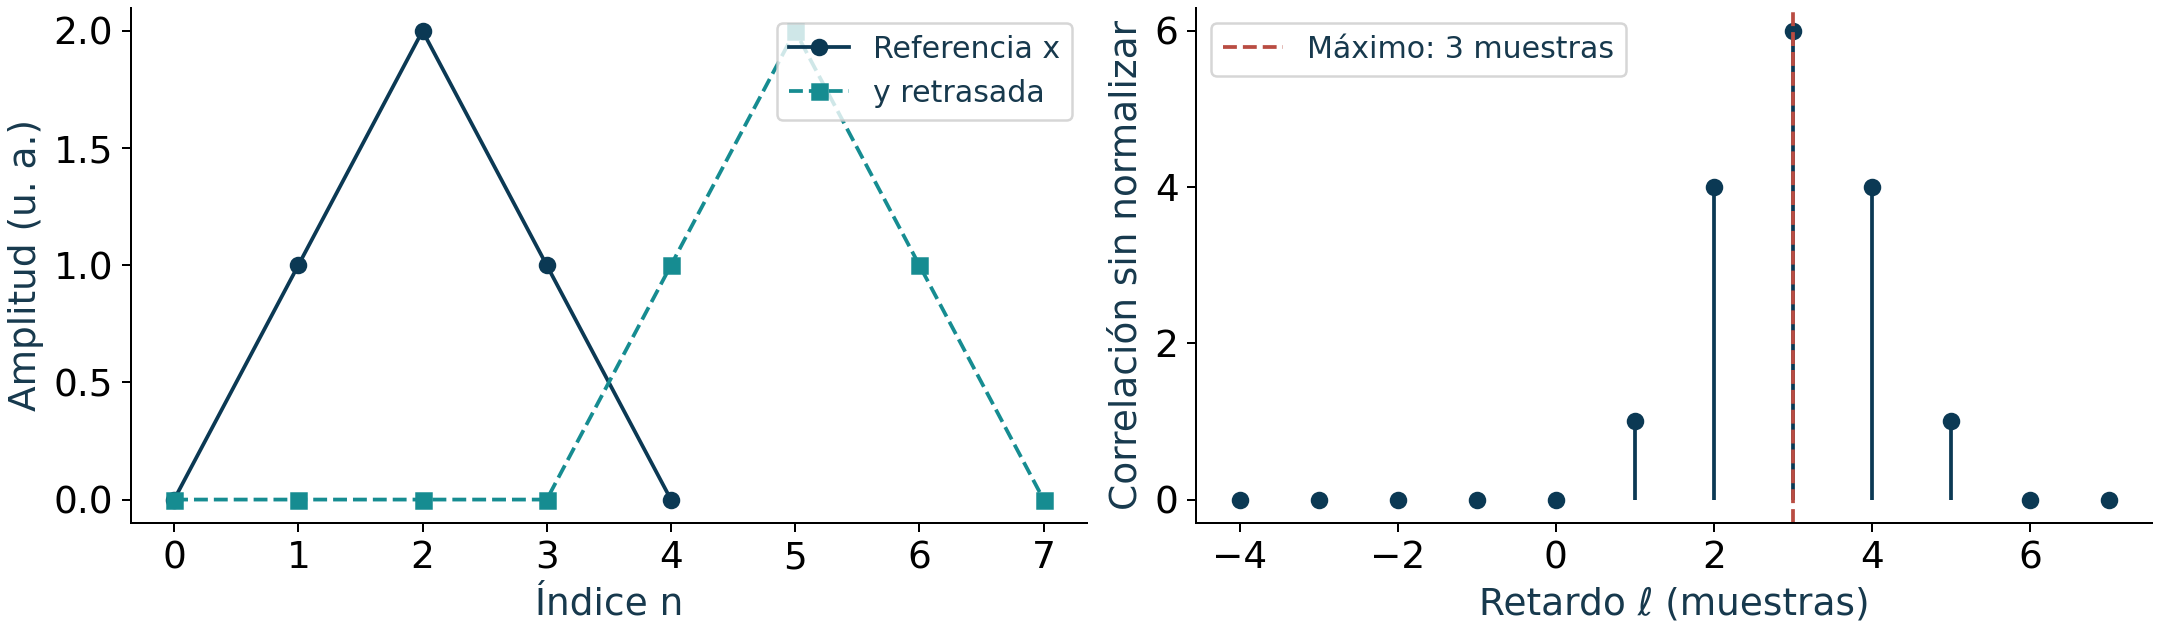
\includegraphics[width=0.95\linewidth,height=\textheight,keepaspectratio]{figuras/correlacion.png}

}

\caption{La simulación muestra un desplazamiento de tres muestras. El
signo corresponde a correlate(y, x).}

\end{figure}%

\note{\textbf{Libro guía:} John Semmlow, \emph{Circuits, Signals, and
Systems for Bioengineers}, 3.ª ed., 2018.

§2.4.4, \textbf{Shifted Correlations: Cross-Correlation} (página 89 del
visor PDF).

\textbf{Correspondencia:} Ejemplo, figura o implementación de
elaboración docente a partir de estos fundamentos. No es una
transcripción del código MATLAB del libro. Figura de cálculo propio con
señales sintéticas. Código reproducible:
codigo/ejemplos\_verificados.py.

\textbf{Microcurrículo:} semana 3, sesión 2 (sesión global 6). Los
numerales del cronograma son identificadores curriculares; no son los
apartados del libro citados arriba.}
\end{frame}

\begin{frame}{Semana 4 · Segmentación, normalización y límites del
tiempo}
\phantomsection\label{d1-061}
\note{\textbf{Libro guía:} John Semmlow, \emph{Circuits, Signals, and
Systems for Bioengineers}, 3.ª ed., 2018.

§1.1, \textbf{Why Biomedical Engineers Need To Analyze Signals And
Systems} (página 8 del visor PDF); §2.2, \textbf{Time Domain
Measurements} (página 57 del visor PDF); §2.4, \textbf{Time Domain
Analysis} (página 81 del visor PDF); §3.3, \textbf{Time--Frequency
Transformation Of Continuous Signals} (página 118 del visor PDF).

\textbf{Correspondencia:} Síntesis o encuadre que reúne varias
secciones; no corresponde a un único apartado del libro.

\textbf{Lectura:} use estas secciones como ruta de preparación y
consulta. La bibliografía aparece al final del bloque.}
\end{frame}

\begin{frame}{Sesión 7 · Segmentar es definir la unidad de análisis}
\phantomsection\label{d1-062}
Formas frecuentes:

\begin{itemize}
\tightlist
\item
  ventanas de longitud fija;
\item
  ventanas solapadas;
\item
  segmentos sincronizados con eventos;
\item
  ciclos fisiológicos completos;
\item
  épocas definidas por el protocolo.
\end{itemize}

\begin{block}{Concepto clave}

La segmentación determina qué variación queda dentro del ejemplo y qué
variación se compara entre ejemplos. Es una decisión analítica, no un
trámite.

\end{block}

\note{\textbf{Libro guía:} John Semmlow, \emph{Circuits, Signals, and
Systems for Bioengineers}, 3.ª ed., 2018.

§2.2.4, \textbf{Ensemble Averaging} (página 70 del visor PDF); §2.4.3,
\textbf{Correlations Between Signals} (página 86 del visor PDF).

\textbf{Correspondencia:} Tema previsto en el cronograma, desarrollado
como ampliación docente. Las referencias del libro son antecedentes
conceptuales. El cronograma prescribe este tema. Las secciones citadas
aportan antecedentes; el libro no dedica una sección específica a cada
técnica de preprocesamiento o detección presentada aquí.

\textbf{Microcurrículo:} semana 4, sesión 1 (sesión global 7). Los
numerales del cronograma son identificadores curriculares; no son los
apartados del libro citados arriba.}
\end{frame}

\begin{frame}{Longitud de ventana: compromiso fundamental}
\phantomsection\label{d1-063}
Ventanas cortas:

\begin{itemize}
\tightlist
\item
  mejor localización temporal;
\item
  menos ciclos observados;
\item
  descriptores más variables.
\end{itemize}

Ventanas largas:

\begin{itemize}
\tightlist
\item
  estimaciones más estables;
\item
  mezclan estados fisiológicos;
\item
  reducen localización temporal.
\end{itemize}

\begin{alertblock}{Atención}

No existe una longitud universal. Debe ser compatible con la escala
temporal del fenómeno y con la hipótesis de estacionariedad local.

\end{alertblock}

\note{\textbf{Libro guía:} John Semmlow, \emph{Circuits, Signals, and
Systems for Bioengineers}, 3.ª ed., 2018.

§4.2.3, \textbf{Data Truncation} (página 184 del visor PDF); §4.6,
\textbf{Time--Frequency Analysis} (página 205 del visor PDF).

\textbf{Correspondencia:} Tema previsto en el cronograma, desarrollado
como ampliación docente. Las referencias del libro son antecedentes
conceptuales. El cronograma prescribe este tema. Las secciones citadas
aportan antecedentes; el libro no dedica una sección específica a cada
técnica de preprocesamiento o detección presentada aquí.

\textbf{Microcurrículo:} semana 4, sesión 1 (sesión global 7). Los
numerales del cronograma son identificadores curriculares; no son los
apartados del libro citados arriba.}
\end{frame}

\begin{frame}{Solapamiento aumenta ejemplos, no información
independiente}
\phantomsection\label{d1-064}
Con longitud \(L\) y avance \(H\):

\[\text{solapamiento}=1-\frac{H}{L}\]

Si \(H=L/2\), el solapamiento es 50 \%.

\begin{alertblock}{Atención}

Ventanas vecinas muy solapadas comparten muestras. Si se reparten
aleatoriamente entre entrenamiento y prueba, aparece fuga de
información.

\end{alertblock}

\note{\textbf{Libro guía:} John Semmlow, \emph{Circuits, Signals, and
Systems for Bioengineers}, 3.ª ed., 2018.

§4.4, \textbf{Spectral Averaging} (página 195 del visor PDF).

\textbf{Correspondencia:} Las secciones aportan el fundamento. La
diapositiva amplía la formulación o precisa condiciones que no se
presentan con idéntica notación en el libro. El solapamiento se trata en
promediado espectral. La fuga entre entrenamiento y prueba es una
ampliación para diseños predictivos.

\textbf{Microcurrículo:} semana 4, sesión 1 (sesión global 7). Los
numerales del cronograma son identificadores curriculares; no son los
apartados del libro citados arriba.}
\end{frame}

\begin{frame}{Segmentar por evento conserva contexto fisiológico}
\phantomsection\label{d1-065}
Para un evento en \(t_k\):

\[x_k(\tau)=x(t_k+\tau),\qquad \tau\in[-T_{pre},T_{post}]\]

Ejemplos:

\begin{itemize}
\tightlist
\item
  épocas EEG alrededor de un estímulo;
\item
  latidos ECG alineados por onda R;
\item
  ciclos de marcha alineados por contacto de talón.
\end{itemize}

\begin{block}{Comprobación}

Alinear permite comparar morfologías, pero transfiere al análisis el
error temporal del detector de eventos.

\end{block}

\note{\textbf{Libro guía:} John Semmlow, \emph{Circuits, Signals, and
Systems for Bioengineers}, 3.ª ed., 2018.

§2.2.4, \textbf{Ensemble Averaging} (página 70 del visor PDF).

\textbf{Correspondencia:} Actividad o interpretación biomédica de
elaboración docente apoyada en las secciones indicadas. El cronograma
prescribe este tema. Las secciones citadas aportan antecedentes; el
libro no dedica una sección específica a cada técnica de
preprocesamiento o detección presentada aquí.

\textbf{Microcurrículo:} semana 4, sesión 1 (sesión global 7). Los
numerales del cronograma son identificadores curriculares; no son los
apartados del libro citados arriba.}
\end{frame}

\begin{frame}{Autocorrelación y repetición temporal}
\phantomsection\label{d1-066}
Para un registro real de \(N\) muestras centrado, extendido con ceros:

\[r_{xx}[\ell]=\sum_nx_0[n+\ell]x_0[n],\qquad
c_{xx}[\ell]=\frac1N r_{xx}[\ell].\]

Los máximos secundarios pueden sugerir repetición a
\(T\approx\ell/f_s\). Excluya \(\ell=0\) al buscar periodos.

\begin{alertblock}{Atención}

La autocorrelación de datos sin centrar contiene el efecto de la media.
Dividir por \(N\) o por \(N-|\ell|\) cambia sesgo y varianza.
Periodicidad aparente, autocorrelación y mecanismo fisiológico son
afirmaciones distintas.

\end{alertblock}

\note{\textbf{Libro guía:} John Semmlow, \emph{Circuits, Signals, and
Systems for Bioengineers}, 3.ª ed., 2018.

§2.4.5, \textbf{Autocorrelation} (página 104 del visor PDF); §2.4.6,
\textbf{Autocovariance And Cross-Covariance} (página 108 del visor PDF).

\textbf{Correspondencia:} El tema se desarrolla en las secciones
indicadas. La redacción es una síntesis docente.

\textbf{Microcurrículo:} semana 4, sesión 1 (sesión global 7). Los
numerales del cronograma son identificadores curriculares; no son los
apartados del libro citados arriba.}
\end{frame}

\begin{frame}{Normalización de amplitud}
\phantomsection\label{d1-067}
\textbf{Estandarización por segmento:}

\[z[n]=\frac{x[n]-\bar{x}}{s_x}\]

\textbf{Escalamiento min--max:}

\[x'[n]=\frac{x[n]-x_{min}}{x_{max}-x_{min}}\]

\textbf{Normalización por referencia:} \(x'[n]=x[n]/x_{ref}\).

\begin{alertblock}{Atención}

La estandarización elimina nivel y escala. Si \(s_x=0\), o
\(x_{max}=x_{min}\), la normalización no está definida: marque el
segmento constante. Use una referencia no nula y documente sus unidades.

\end{alertblock}

\note{\textbf{Libro guía:} John Semmlow, \emph{Circuits, Signals, and
Systems for Bioengineers}, 3.ª ed., 2018.

§2.2.4, \textbf{Ensemble Averaging} (página 70 del visor PDF); §2.4.3,
\textbf{Correlations Between Signals} (página 86 del visor PDF).

\textbf{Correspondencia:} Tema previsto en el cronograma, desarrollado
como ampliación docente. Las referencias del libro son antecedentes
conceptuales. El cronograma prescribe este tema. Las secciones citadas
aportan antecedentes; el libro no dedica una sección específica a cada
técnica de preprocesamiento o detección presentada aquí.

\textbf{Microcurrículo:} semana 4, sesión 1 (sesión global 7). Los
numerales del cronograma son identificadores curriculares; no son los
apartados del libro citados arriba.}
\end{frame}

\begin{frame}{Normalización fisiológica: ventajas y riesgos}
\phantomsection\label{d1-068}
Ejemplos:

\begin{itemize}
\tightlist
\item
  EMG como porcentaje de contracción voluntaria de referencia;
\item
  ciclo de marcha expresado de 0 \% a 100 \%;
\item
  presión relativa a línea base;
\item
  PPG normalizada por componente lenta.
\end{itemize}

\begin{block}{Concepto clave}

Una referencia inestable transmite su error a todos los datos
normalizados. Deben registrarse protocolo, repetibilidad y criterio de
selección.

\end{block}

\note{\textbf{Libro guía:} John Semmlow, \emph{Circuits, Signals, and
Systems for Bioengineers}, 3.ª ed., 2018.

§2.2.4, \textbf{Ensemble Averaging} (página 70 del visor PDF); §2.4.3,
\textbf{Correlations Between Signals} (página 86 del visor PDF).

\textbf{Correspondencia:} Tema previsto en el cronograma, desarrollado
como ampliación docente. Las referencias del libro son antecedentes
conceptuales. El cronograma prescribe este tema. Las secciones citadas
aportan antecedentes; el libro no dedica una sección específica a cada
técnica de preprocesamiento o detección presentada aquí.

\textbf{Microcurrículo:} semana 4, sesión 1 (sesión global 7). Los
numerales del cronograma son identificadores curriculares; no son los
apartados del libro citados arriba.}
\end{frame}

\begin{frame}{Evitar fuga de información en normalización}
\phantomsection\label{d1-069}
Procedimiento correcto para aprendizaje automático:

\begin{enumerate}
\tightlist
\item
  dividir por sujeto o unidad independiente;
\item
  estimar media, desviación u otros parámetros \textbf{solo en
  entrenamiento};
\item
  aplicar esos parámetros sin reajuste a validación y prueba.
\end{enumerate}

\begin{alertblock}{Atención}

Esta regla se aplica a parámetros aprendidos del conjunto. Una
transformación fija por segmento puede calcularse sobre ese segmento si
coincide con el uso previsto; en tiempo real no debe utilizar muestras
futuras.

\end{alertblock}

\note{\textbf{Libro guía:} John Semmlow, \emph{Circuits, Signals, and
Systems for Bioengineers}, 3.ª ed., 2018.

§2.4.3, \textbf{Correlations Between Signals} (página 86 del visor PDF).

\textbf{Correspondencia:} No existe una sección específica del libro
guía para el tema completo de esta diapositiva. Las secciones anteriores
son antecedentes, no referencias directas. No hay sección específica de
partición de conjuntos en el libro guía. Complemento conceptual: Semmlow
y Griffel (2014), §16.1.1 y §16.6. Desarrollo docente sobre separación
por sujeto.

\textbf{Microcurrículo:} semana 4, sesión 1 (sesión global 7). Los
numerales del cronograma son identificadores curriculares; no son los
apartados del libro citados arriba.}
\end{frame}

\begin{frame}{Lista de control de un segmento analizable}
\phantomsection\label{d1-070}
\begin{itemize}
\tightlist
\item
  ¿Tiene sello temporal y frecuencia de muestreo?
\item
  ¿Conserva unidades y calibración?
\item
  ¿Contiene valores faltantes o saturación?
\item
  ¿Su longitud está justificada?
\item
  ¿La etiqueta se definió sin usar información futura?
\item
  ¿Pertenece a un sujeto ya presente en otro subconjunto?
\end{itemize}

\begin{block}{Evidencia mínima}

Guardar índices inicial/final, regla de segmentación, parámetros de
normalización y relación con el registro original.

\end{block}

\note{\textbf{Libro guía:} John Semmlow, \emph{Circuits, Signals, and
Systems for Bioengineers}, 3.ª ed., 2018.

§2.2.4, \textbf{Ensemble Averaging} (página 70 del visor PDF); §2.4.3,
\textbf{Correlations Between Signals} (página 86 del visor PDF).

\textbf{Correspondencia:} Tema previsto en el cronograma, desarrollado
como ampliación docente. Las referencias del libro son antecedentes
conceptuales. El cronograma prescribe este tema. Las secciones citadas
aportan antecedentes; el libro no dedica una sección específica a cada
técnica de preprocesamiento o detección presentada aquí.

\textbf{Microcurrículo:} semana 4, sesión 1 (sesión global 7). Los
numerales del cronograma son identificadores curriculares; no son los
apartados del libro citados arriba.}
\end{frame}

\begin{frame}{Sesión 8 · El dominio temporal puede ocultar estructura}
\phantomsection\label{d1-071}
Dos señales pueden tener:

\begin{itemize}
\tightlist
\item
  media y RMS similares;
\item
  amplitud comparable;
\item
  duración igual;
\end{itemize}

pero oscilaciones dominantes distintas.

\begin{block}{Concepto clave}

El dominio temporal responde bien ``cuándo'' y ``cuánto''. El dominio
frecuencial ayuda a responder ``a qué ritmos'' se distribuye la
variación.

\end{block}

\note{\textbf{Libro guía:} John Semmlow, \emph{Circuits, Signals, and
Systems for Bioengineers}, 3.ª ed., 2018.

§2.4, \textbf{Time Domain Analysis} (página 81 del visor PDF); §3.2,
\textbf{Time--Frequency Domains: General Concepts} (página 117 del visor
PDF).

\textbf{Correspondencia:} El tema se desarrolla en las secciones
indicadas. La redacción es una síntesis docente.

\textbf{Microcurrículo:} semana 4, sesión 2 (sesión global 8). Los
numerales del cronograma son identificadores curriculares; no son los
apartados del libro citados arriba.}
\end{frame}

\begin{frame}{Frecuencia como tasa de repetición}
\phantomsection\label{d1-072}
\[f=\frac{1}{T},\qquad \omega=2\pi f\]

Interpretaciones:

\begin{itemize}
\tightlist
\item
  respiración a 0.25 Hz: un ciclo cada 4 s;
\item
  oscilación a 10 Hz: diez ciclos por segundo;
\item
  componente DC: frecuencia 0 Hz, asociada al promedio.
\end{itemize}

\begin{alertblock}{Atención}

Una frecuencia presente en el registro no identifica por sí sola su
origen: puede ser fisiológica, instrumental o artefactual.

\end{alertblock}

\note{\textbf{Libro guía:} John Semmlow, \emph{Circuits, Signals, and
Systems for Bioengineers}, 3.ª ed., 2018.

§2.3.1, \textbf{Sinusoids As Real-Valued Signals} (página 73 del visor
PDF); §3.3.1, \textbf{Sinusoidal Properties In The Time And Frequency
Domains} (página 118 del visor PDF).

\textbf{Correspondencia:} El tema se desarrolla en las secciones
indicadas. La redacción es una síntesis docente.

\textbf{Microcurrículo:} semana 4, sesión 2 (sesión global 8). Los
numerales del cronograma son identificadores curriculares; no son los
apartados del libro citados arriba.}
\end{frame}

\begin{frame}{Ortogonalidad: fundamento de la descomposición}
\phantomsection\label{d1-073}
Dos funciones son ortogonales sobre el intervalo elegido si:

\[\langle x,y\rangle=\int_{t_0}^{t_0+T_0}x(t)y^*(t)\,dt=0.\]

Senos y cosenos armónicos tienen esta propiedad al integrar sobre un
periodo común completo.

\begin{block}{Concepto clave}

Ortogonalidad significa producto interno nulo. Correlación de Pearson
nula se refiere a señales centradas. Ambas nociones coinciden solo bajo
las condiciones adecuadas de centrado y normalización.

\end{block}

\textbf{Puente a Fourier:} cada coeficiente mide una proyección sobre
una función de la base.

\note{\textbf{Libro guía:} John Semmlow, \emph{Circuits, Signals, and
Systems for Bioengineers}, 3.ª ed., 2018.

§2.4.2, \textbf{Orthogonal Signals And Orthogonality} (página 86 del
visor PDF); §3.3.4, \textbf{Finding The Fourier Coefficients} (página
123 del visor PDF).

\textbf{Correspondencia:} El tema se desarrolla en las secciones
indicadas. La redacción es una síntesis docente.

\textbf{Microcurrículo:} semana 4, sesión 2 (sesión global 8). Los
numerales del cronograma son identificadores curriculares; no son los
apartados del libro citados arriba.}
\end{frame}

\begin{frame}{Una señal compleja puede verse como suma de oscilaciones}
\phantomsection\label{d1-074}
Modelo conceptual:

\[x(t)=\sum_k A_k\cos(2\pi f_kt+\phi_k)\]

El análisis frecuencial busca estimar:

\begin{itemize}
\tightlist
\item
  qué frecuencias \(f_k\) participan;
\item
  con qué amplitudes \(A_k\);
\item
  con qué fases \(\phi_k\);
\item
  cómo cambian con el tiempo.
\end{itemize}

\begin{block}{Nota}

La suma de sinusoides no implica que el organismo posea ``osciladores
puros''; es una base matemática para representar el registro.

\end{block}

\note{\textbf{Libro guía:} John Semmlow, \emph{Circuits, Signals, and
Systems for Bioengineers}, 3.ª ed., 2018.

§3.3.2, \textbf{Sinusoidal Decomposition: The Fourier Series} (página
119 del visor PDF).

\textbf{Correspondencia:} El tema se desarrolla en las secciones
indicadas. La redacción es una síntesis docente.

\textbf{Microcurrículo:} semana 4, sesión 2 (sesión global 8). Los
numerales del cronograma son identificadores curriculares; no son los
apartados del libro citados arriba.}
\end{frame}

\begin{frame}{Tiempo y frecuencia son representaciones complementarias}
\phantomsection\label{d1-075}
\begin{longtable}[]{@{}
  >{\raggedright\arraybackslash}p{(\linewidth - 2\tabcolsep) * \real{0.5000}}
  >{\raggedright\arraybackslash}p{(\linewidth - 2\tabcolsep) * \real{0.5000}}@{}}
\toprule\noalign{}
\begin{minipage}[b]{\linewidth}\raggedright
Dominio temporal
\end{minipage} & \begin{minipage}[b]{\linewidth}\raggedright
Dominio frecuencial
\end{minipage} \\
\midrule\noalign{}
\endhead
localiza transitorios y eventos & separa ritmos superpuestos \\
muestra morfología & resume distribución por frecuencia \\
facilita alineación fisiológica & permite estudiar banda y resonancia \\
puede ocultar periodicidades débiles & magnitud o PSD global no
localizan eventos \\
\bottomrule\noalign{}
\end{longtable}

\begin{block}{Concepto clave}

La transformada compleja completa es invertible bajo sus condiciones de
existencia. Lo que pierde localización explícita es un resumen global
como magnitud o PSD. La estacionariedad se refiere al modelo
estadístico, no a la posibilidad de calcular Fourier.

\end{block}

\note{\textbf{Libro guía:} John Semmlow, \emph{Circuits, Signals, and
Systems for Bioengineers}, 3.ª ed., 2018.

§3.2, \textbf{Time--Frequency Domains: General Concepts} (página 117 del
visor PDF); §3.3.7, \textbf{The Continuous Fourier Transform} (página
138 del visor PDF).

\textbf{Correspondencia:} El tema se desarrolla en las secciones
indicadas. La redacción es una síntesis docente.

\textbf{Microcurrículo:} semana 4, sesión 2 (sesión global 8). Los
numerales del cronograma son identificadores curriculares; no son los
apartados del libro citados arriba.}
\end{frame}

\begin{frame}{Estacionariedad: el supuesto que suele quedar oculto}
\phantomsection\label{d1-076}
Un proceso aleatorio \(x(t)\), con segundo momento finito, es
estacionario en sentido amplio si:

\[\mathbb{E}\{x(t)\}=\mu\quad\text{constante}\]

\[R_x(t_1,t_2)=R_x(t_1-t_2)\]

En práctica se habla de \textbf{estacionariedad local} en ventanas donde
propiedades relevantes cambian poco.

\begin{alertblock}{Atención}

Un único espectro global puede mezclar reposo, movimiento, transición y
artefacto, produciendo una descripción sin estado fisiológico claro.

\end{alertblock}

\note{\textbf{Libro guía:} John Semmlow, \emph{Circuits, Signals, and
Systems for Bioengineers}, 3.ª ed., 2018.

§10.2, \textbf{Stochastic Processes: Stationarity And Ergodicity}
(página 450 del visor PDF).

\textbf{Correspondencia:} Las secciones aportan el fundamento. La
diapositiva amplía la formulación o precisa condiciones que no se
presentan con idéntica notación en el libro. La estacionariedad se
desarrolla en el capítulo 10 del libro guía, fuera del núcleo de
capítulos 1--8. Se anticipa para justificar ventanas del cronograma.

\textbf{Microcurrículo:} semana 4, sesión 2 (sesión global 8). Los
numerales del cronograma son identificadores curriculares; no son los
apartados del libro citados arriba.}
\end{frame}

\begin{frame}{Preparación responsable antes del espectro}
\phantomsection\label{d1-077}
\begin{enumerate}
\tightlist
\item
  verificar frecuencia de muestreo y tiempo;
\item
  revisar saturación y faltantes;
\item
  seleccionar un segmento coherente;
\item
  decidir si retirar media o tendencia;
\item
  documentar unidades y preprocesamiento;
\item
  anticipar duración y resolución requeridas.
\end{enumerate}

\begin{block}{Comprobación}

El espectro no corrige una adquisición deficiente. Solo reorganiza la
información contenida en el registro disponible.

\end{block}

\note{\textbf{Libro guía:} John Semmlow, \emph{Circuits, Signals, and
Systems for Bioengineers}, 3.ª ed., 2018.

§4.2, \textbf{Data Acquisition And Storage} (página 175 del visor PDF);
§4.6, \textbf{Time--Frequency Analysis} (página 205 del visor PDF).

\textbf{Correspondencia:} Actividad o interpretación biomédica de
elaboración docente apoyada en las secciones indicadas.

\textbf{Microcurrículo:} semana 4, sesión 2 (sesión global 8). Los
numerales del cronograma son identificadores curriculares; no son los
apartados del libro citados arriba.}
\end{frame}

\begin{frame}{Verificación de la semana 4}
\phantomsection\label{d1-078}
Se registran 60 s de PPG durante una transición de reposo a ejercicio.

\begin{enumerate}
\tightlist
\item
  ¿Sería defendible un único espectro de 60 s?
\item
  ¿Qué ventanas usaría y por qué?
\item
  ¿Qué canal auxiliar ayudaría a identificar artefactos?
\item
  ¿Qué normalización conservaría información de amplitud?
\item
  ¿Cómo evitaría fuga entre entrenamiento y prueba?
\end{enumerate}

\begin{block}{Criterio de logro}

La propuesta debe enlazar escala fisiológica, estacionariedad local,
dependencia entre ventanas y objetivo del análisis.

\end{block}

\note{\textbf{Libro guía:} John Semmlow, \emph{Circuits, Signals, and
Systems for Bioengineers}, 3.ª ed., 2018.

§2.2.4, \textbf{Ensemble Averaging} (página 70 del visor PDF); §4.6,
\textbf{Time--Frequency Analysis} (página 205 del visor PDF); §10.2,
\textbf{Stochastic Processes: Stationarity And Ergodicity} (página 450
del visor PDF).

\textbf{Correspondencia:} Actividad o interpretación biomédica de
elaboración docente apoyada en las secciones indicadas.

\textbf{Microcurrículo:} semana 4, sesión 2 (sesión global 8). Los
numerales del cronograma son identificadores curriculares; no son los
apartados del libro citados arriba.}
\end{frame}

\begin{frame}{Semana 5 · De la periodicidad al espectro}
\phantomsection\label{d1-079}
\note{\textbf{Libro guía:} John Semmlow, \emph{Circuits, Signals, and
Systems for Bioengineers}, 3.ª ed., 2018.

§1.1, \textbf{Why Biomedical Engineers Need To Analyze Signals And
Systems} (página 8 del visor PDF); §2.2, \textbf{Time Domain
Measurements} (página 57 del visor PDF); §2.4, \textbf{Time Domain
Analysis} (página 81 del visor PDF); §3.3, \textbf{Time--Frequency
Transformation Of Continuous Signals} (página 118 del visor PDF).

\textbf{Correspondencia:} Síntesis o encuadre que reúne varias
secciones; no corresponde a un único apartado del libro.

\textbf{Lectura:} use estas secciones como ruta de preparación y
consulta. La bibliografía aparece al final del bloque.}
\end{frame}

\begin{frame}{Sesión 9 · Una señal periódica se repite}
\phantomsection\label{d1-080}
\[x(t+T_0)=x(t)\]

El menor \(T_0>0\) que satisface la igualdad es el periodo fundamental.
Su frecuencia fundamental es:

\[f_0=\frac{1}{T_0},\qquad \omega_0=\frac{2\pi}{T_0}\]

\begin{alertblock}{Atención}

Que un patrón parezca repetirse durante pocos ciclos no demuestra
periodicidad matemática. Las bioseñales suelen ser cuasiperiódicas.

\end{alertblock}

\note{\textbf{Libro guía:} John Semmlow, \emph{Circuits, Signals, and
Systems for Bioengineers}, 3.ª ed., 2018.

§1.4.2, \textbf{Deterministic Signal Properties: Periodic, Aperiodic,
And Transient} (página 37 del visor PDF); §3.3.2, \textbf{Sinusoidal
Decomposition: The Fourier Series} (página 119 del visor PDF).

\textbf{Correspondencia:} El tema se desarrolla en las secciones
indicadas. La redacción es una síntesis docente.

\textbf{Microcurrículo:} semana 5, sesión 1 (sesión global 9). Los
numerales del cronograma son identificadores curriculares; no son los
apartados del libro citados arriba.}
\end{frame}

\begin{frame}{Armónicos: múltiplos de la frecuencia fundamental}
\phantomsection\label{d1-081}
\[f_k=kf_0,\qquad k\in\mathbb{Z}\]

\begin{itemize}
\tightlist
\item
  \(k=0\): componente DC.
\item
  \(k=1\): fundamental.
\item
  \(k=2,3,\ldots\): armónicos.
\end{itemize}

\begin{block}{Concepto clave}

La frecuencia fundamental describe repetición; los armónicos permiten
reconstruir detalles de forma dentro de cada periodo.

\end{block}

\note{\textbf{Libro guía:} John Semmlow, \emph{Circuits, Signals, and
Systems for Bioengineers}, 3.ª ed., 2018.

§3.3.2, \textbf{Sinusoidal Decomposition: The Fourier Series} (página
119 del visor PDF).

\textbf{Correspondencia:} El tema se desarrolla en las secciones
indicadas. La redacción es una síntesis docente.

\textbf{Microcurrículo:} semana 5, sesión 1 (sesión global 9). Los
numerales del cronograma son identificadores curriculares; no son los
apartados del libro citados arriba.}
\end{frame}

\begin{frame}{Serie trigonométrica de Fourier}
\phantomsection\label{d1-082}
\[x(t)=a_0+\sum_{k=1}^{\infty}
\left[a_k\cos(k\omega_0t)+b_k\sin(k\omega_0t)\right]\]

Los coeficientes miden la proyección de la señal sobre cada senoide
armónica.

\begin{block}{Concepto clave}

Para señales periódicas de energía finita por periodo, la serie converge
en media cuadrática. Bajo condiciones de Dirichlet, en un salto converge
al promedio de los límites laterales. Los armónicos son una
representación matemática.

\end{block}

\note{\textbf{Libro guía:} John Semmlow, \emph{Circuits, Signals, and
Systems for Bioengineers}, 3.ª ed., 2018.

§3.3.4, \textbf{Finding The Fourier Coefficients} (página 123 del visor
PDF).

\textbf{Correspondencia:} El tema se desarrolla en las secciones
indicadas. La redacción es una síntesis docente.

\textbf{Microcurrículo:} semana 5, sesión 1 (sesión global 9). Los
numerales del cronograma son identificadores curriculares; no son los
apartados del libro citados arriba.}
\end{frame}

\begin{frame}{Los coeficientes cuantifican cada armónico}
\phantomsection\label{d1-083}
\[a_0=\frac{1}{T_0}\int_{T_0}x(t)\,dt\]

\[a_k=\frac{2}{T_0}\int_{T_0}x(t)\cos(k\omega_0t)\,dt\]

\[b_k=\frac{2}{T_0}\int_{T_0}x(t)\sin(k\omega_0t)\,dt\]

\textbf{Convención:} algunos textos escriben \(a_0/2\); debe conservarse
una notación consistente.

\note{\textbf{Libro guía:} John Semmlow, \emph{Circuits, Signals, and
Systems for Bioengineers}, 3.ª ed., 2018.

§3.3.4, \textbf{Finding The Fourier Coefficients} (página 123 del visor
PDF).

\textbf{Correspondencia:} El tema se desarrolla en las secciones
indicadas. La redacción es una síntesis docente.

\textbf{Microcurrículo:} semana 5, sesión 1 (sesión global 9). Los
numerales del cronograma son identificadores curriculares; no son los
apartados del libro citados arriba.}
\end{frame}

\begin{frame}{Forma compleja de la serie}
\phantomsection\label{d1-084}
\[x(t)=\sum_{k=-\infty}^{\infty}c_ke^{jk\omega_0t}\]

\[c_k=\frac{1}{T_0}\int_{T_0}x(t)e^{-jk\omega_0t}\,dt\]

Relación con la forma trigonométrica para \(k>0\):

\[c_k=\frac{a_k-jb_k}{2},\qquad c_{-k}=c_k^*\]

\begin{block}{Concepto clave}

En señales reales, \(c_{-k}=c_k^*\) vincula frecuencias positivas y
negativas.

\end{block}

\note{\textbf{Libro guía:} John Semmlow, \emph{Circuits, Signals, and
Systems for Bioengineers}, 3.ª ed., 2018.

§3.3.6, \textbf{Complex Representation} (página 132 del visor PDF).

\textbf{Correspondencia:} El tema se desarrolla en las secciones
indicadas. La redacción es una síntesis docente.

\textbf{Microcurrículo:} semana 5, sesión 1 (sesión global 9). Los
numerales del cronograma son identificadores curriculares; no son los
apartados del libro citados arriba.}
\end{frame}

\begin{frame}{Simetría reduce el trabajo}
\phantomsection\label{d1-085}
\begin{itemize}
\tightlist
\item
  Si \(x(t)\) es \textbf{par}, \(x(-t)=x(t)\): desaparecen los términos
  seno.
\item
  Si \(x(t)\) es \textbf{impar}, \(x(-t)=-x(t)\): desaparecen DC y
  términos coseno.
\item
  Si no hay simetría, se requieren ambos conjuntos.
\end{itemize}

\begin{block}{Comprobación}

Antes de integrar, inspeccione simetría y elija un intervalo de longitud
\(T_0\) que simplifique el cálculo.

\end{block}

\note{\textbf{Libro guía:} John Semmlow, \emph{Circuits, Signals, and
Systems for Bioengineers}, 3.ª ed., 2018.

§3.3.5, \textbf{Symmetry} (página 127 del visor PDF).

\textbf{Correspondencia:} El tema se desarrolla en las secciones
indicadas. La redacción es una síntesis docente.

\textbf{Microcurrículo:} semana 5, sesión 1 (sesión global 9). Los
numerales del cronograma son identificadores curriculares; no son los
apartados del libro citados arriba.}
\end{frame}

\begin{frame}{Ejemplo conceptual: pulso periódico}
\phantomsection\label{d1-086}
Una forma con transiciones abruptas requiere muchos armónicos para
aproximarse.

\begin{itemize}
\tightlist
\item
  pocos armónicos: conserva tendencia y forma gruesa;
\item
  más armónicos: mejora bordes y detalles;
\item
  cerca de discontinuidades persiste sobreoscilación de Gibbs.
\end{itemize}

\begin{alertblock}{Atención}

Agregar armónicos no elimina completamente el sobreimpulso porcentual en
una discontinuidad; estrecha la región donde ocurre.

\end{alertblock}

\note{\textbf{Libro guía:} John Semmlow, \emph{Circuits, Signals, and
Systems for Bioengineers}, 3.ª ed., 2018.

§3.3.4, \textbf{Finding The Fourier Coefficients} (página 123 del visor
PDF); §3.4.4, \textbf{The Inverse Discrete Fourier Transform} (página
163 del visor PDF).

\textbf{Correspondencia:} Actividad o interpretación biomédica de
elaboración docente apoyada en las secciones indicadas.

\textbf{Microcurrículo:} semana 5, sesión 1 (sesión global 9). Los
numerales del cronograma son identificadores curriculares; no son los
apartados del libro citados arriba.}
\end{frame}

\begin{frame}{Parseval conecta tiempo y armónicos}
\phantomsection\label{d1-087}
Para la serie compleja:

\[\frac{1}{T_0}\int_{T_0}|x(t)|^2dt
=\sum_{k=-\infty}^{\infty}|c_k|^2\]

\begin{block}{Concepto clave}

La potencia media calculada en el tiempo coincide con la suma de
contribuciones cuadráticas de los coeficientes espectrales.

\end{block}

\note{\textbf{Libro guía:} John Semmlow, \emph{Circuits, Signals, and
Systems for Bioengineers}, 3.ª ed., 2018.

§3.3.4, \textbf{Finding The Fourier Coefficients} (página 123 del visor
PDF); §4.3, \textbf{Power Spectrum} (página 191 del visor PDF).

\textbf{Correspondencia:} Las secciones aportan el fundamento. La
diapositiva amplía la formulación o precisa condiciones que no se
presentan con idéntica notación en el libro.

\textbf{Microcurrículo:} semana 5, sesión 1 (sesión global 9). Los
numerales del cronograma son identificadores curriculares; no son los
apartados del libro citados arriba.}
\end{frame}

\begin{frame}{Reconstrucción truncada}
\phantomsection\label{d1-088}
\[x_K(t)=\sum_{k=-K}^{K}c_ke^{jk\omega_0t}\]

Preguntas de interpretación:

\begin{itemize}
\tightlist
\item
  ¿qué rasgos morfológicos aparecen primero?
\item
  ¿cuántos armónicos se necesitan para la pregunta biomédica?
\item
  ¿el error se distribuye uniformemente?
\end{itemize}

\begin{block}{Nota}

La mejor reconstrucción matemática no siempre es la representación más
útil. Puede bastar una banda limitada para un rasgo específico.

\end{block}

\note{\textbf{Libro guía:} John Semmlow, \emph{Circuits, Signals, and
Systems for Bioengineers}, 3.ª ed., 2018.

§3.3.4, \textbf{Finding The Fourier Coefficients} (página 123 del visor
PDF); §3.4.4, \textbf{The Inverse Discrete Fourier Transform} (página
163 del visor PDF).

\textbf{Correspondencia:} Actividad o interpretación biomédica de
elaboración docente apoyada en las secciones indicadas.

\textbf{Microcurrículo:} semana 5, sesión 1 (sesión global 9). Los
numerales del cronograma son identificadores curriculares; no son los
apartados del libro citados arriba.}
\end{frame}

\begin{frame}{Pulso periódico: coeficientes calculados}
\phantomsection\label{d1-089}
Para un pulso de amplitud \(A\), centrado, ancho \(\tau\) y periodo
\(T_0\), defina \(D=\tau/T_0\):

\[c_k=\frac{A}{T_0}\int_{-\tau/2}^{\tau/2}e^{-j2\pi kt/T_0}dt
=AD\,\mathrm{sinc}(kD).\]

Con \(D=1/2\): \(c_0=A/2\), \(c_1=A/\pi\) y \(c_2=0\).

\begin{block}{Comprobación}

La componente continua coincide con amplitud por ciclo de trabajo. Use
simetría y unidades para comprobar el resultado antes de reconstruir.

\end{block}

\note{\textbf{Libro guía:} John Semmlow, \emph{Circuits, Signals, and
Systems for Bioengineers}, 3.ª ed., 2018.

§3.3.4, \textbf{Finding The Fourier Coefficients} (página 123 del visor
PDF); §3.3.5, \textbf{Symmetry} (página 127 del visor PDF).

\textbf{Correspondencia:} Ejemplo, figura o implementación de
elaboración docente a partir de estos fundamentos. No es una
transcripción del código MATLAB del libro. Ejemplo didáctico original,
no reproducción de un ejercicio del libro.

\textbf{Microcurrículo:} semana 5, sesión 1 (sesión global 9). Los
numerales del cronograma son identificadores curriculares; no son los
apartados del libro citados arriba.}
\end{frame}

\begin{frame}{Reconstrucción y discontinuidades}
\phantomsection\label{d1-090}
\begin{figure}[H]

{\centering 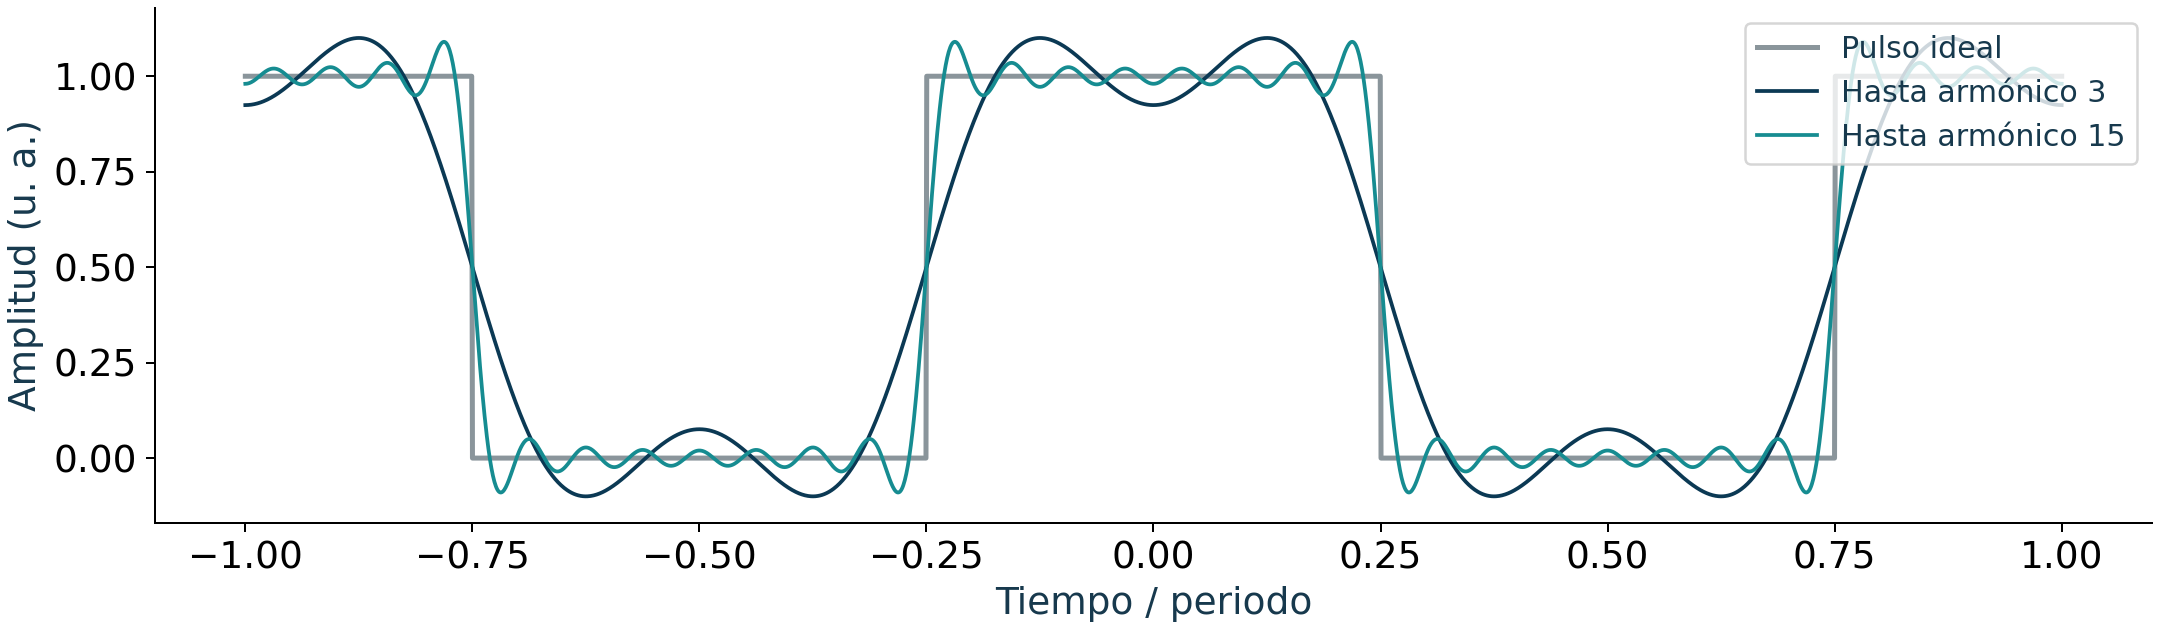
\includegraphics[width=0.95\linewidth,height=\textheight,keepaspectratio]{figuras/fourier-pulso.png}

}

\caption{Pulso sintético de ciclo de trabajo 1/2. Aumentar armónicos
estrecha la región de Gibbs, pero no elimina su sobreimpulso relativo.}

\end{figure}%

\note{\textbf{Libro guía:} John Semmlow, \emph{Circuits, Signals, and
Systems for Bioengineers}, 3.ª ed., 2018.

§3.3.4, \textbf{Finding The Fourier Coefficients} (página 123 del visor
PDF); §3.3.5, \textbf{Symmetry} (página 127 del visor PDF).

\textbf{Correspondencia:} Ejemplo, figura o implementación de
elaboración docente a partir de estos fundamentos. No es una
transcripción del código MATLAB del libro. Figura de cálculo propio con
señales sintéticas. Código reproducible:
codigo/ejemplos\_verificados.py.

\textbf{Microcurrículo:} semana 5, sesión 1 (sesión global 9). Los
numerales del cronograma son identificadores curriculares; no son los
apartados del libro citados arriba.}
\end{frame}

\begin{frame}{Sesión 10 · De la serie a la transformada de Fourier}
\phantomsection\label{d1-091}
Al aumentar el periodo \(T_0\), el espaciado armónico \(\Delta f=1/T_0\)
disminuye. En el límite aparece un continuo de frecuencias:

\[X(f)=\int_{-\infty}^{\infty}x(t)e^{-j2\pi ft}\,dt\]

Transformada inversa:

\[x(t)=\int_{-\infty}^{\infty}X(f)e^{j2\pi ft}\,df\]

\begin{block}{Concepto clave}

La transformada representa señales aperiódicas mediante un continuo de
frecuencias complejas.

\end{block}

\note{\textbf{Libro guía:} John Semmlow, \emph{Circuits, Signals, and
Systems for Bioengineers}, 3.ª ed., 2018.

§3.3.7, \textbf{The Continuous Fourier Transform} (página 138 del visor
PDF).

\textbf{Correspondencia:} El tema se desarrolla en las secciones
indicadas. La redacción es una síntesis docente.

\textbf{Microcurrículo:} semana 5, sesión 2 (sesión global 10). Los
numerales del cronograma son identificadores curriculares; no son los
apartados del libro citados arriba.}
\end{frame}

\begin{frame}{Magnitud y fase cumplen funciones distintas}
\phantomsection\label{d1-092}
\[X(f)=|X(f)|e^{j\angle X(f)}\]

\begin{itemize}
\tightlist
\item
  \(|X(f)|\): contribución relativa por frecuencia.
\item
  \(\angle X(f)\): alineación temporal de esas componentes.
\end{itemize}

\begin{alertblock}{Atención}

La magnitud sola no determina la morfología temporal. Dos señales pueden
compartir magnitud espectral y diferir notablemente por su fase.

\end{alertblock}

\note{\textbf{Libro guía:} John Semmlow, \emph{Circuits, Signals, and
Systems for Bioengineers}, 3.ª ed., 2018.

§3.3.6, \textbf{Complex Representation} (página 132 del visor PDF);
§3.4.3, \textbf{Details Of The Dft Spectrum} (página 153 del visor PDF).

\textbf{Correspondencia:} El tema se desarrolla en las secciones
indicadas. La redacción es una síntesis docente.

\textbf{Microcurrículo:} semana 5, sesión 2 (sesión global 10). Los
numerales del cronograma son identificadores curriculares; no son los
apartados del libro citados arriba.}
\end{frame}

\begin{frame}{Simetría para señales reales}
\phantomsection\label{d1-093}
Si \(x(t)\in\mathbb{R}\):

\[X(-f)=X^*(f)\]

Por tanto:

\[|X(-f)|=|X(f)|,\qquad \angle X(-f)=-\angle X(f)\]

\begin{block}{Nota}

La fase puede presentar saltos por envoltura en \((-\pi,\pi]\). La
aparente discontinuidad no siempre representa un cambio físico.

\end{block}

\note{\textbf{Libro guía:} John Semmlow, \emph{Circuits, Signals, and
Systems for Bioengineers}, 3.ª ed., 2018.

§3.3.5, \textbf{Symmetry} (página 127 del visor PDF); §3.3.6,
\textbf{Complex Representation} (página 132 del visor PDF).

\textbf{Correspondencia:} El tema se desarrolla en las secciones
indicadas. La redacción es una síntesis docente.

\textbf{Microcurrículo:} semana 5, sesión 2 (sesión global 10). Los
numerales del cronograma son identificadores curriculares; no son los
apartados del libro citados arriba.}
\end{frame}

\begin{frame}{Pares esenciales de transformada}
\phantomsection\label{d1-094}
\begin{longtable}[]{@{}ll@{}}
\toprule\noalign{}
Señal & Transformada \\
\midrule\noalign{}
\endhead
\(\delta(t)\) & \(1\) \\
\(1\) & \(\delta(f)\) \\
\(e^{j2\pi f_0t}\) & \(\delta(f-f_0)\) \\
\(\cos(2\pi f_0t)\) & \(\tfrac12[\delta(f-f_0)+\delta(f+f_0)]\) \\
\(\mathrm{rect}(t/T)\) & \(T\,\mathrm{sinc}(Tf)\) \\
\bottomrule\noalign{}
\end{longtable}

\begin{alertblock}{Atención}

Los pares con constantes, impulsos o sinusoides persistentes se
interpretan como distribuciones. Aquí
\(\mathrm{sinc}(u)=\sin(\pi u)/(\pi u)\), con \(\mathrm{sinc}(0)=1\) y
\(T>0\).

\end{alertblock}

\note{\textbf{Libro guía:} John Semmlow, \emph{Circuits, Signals, and
Systems for Bioengineers}, 3.ª ed., 2018.

§3.3.7, \textbf{The Continuous Fourier Transform} (página 138 del visor
PDF).

\textbf{Correspondencia:} Las secciones aportan el fundamento. La
diapositiva amplía la formulación o precisa condiciones que no se
presentan con idéntica notación en el libro. La diapositiva formaliza
propiedades de la transformada continua. No supone que la tabla o la
notación coincidan literalmente con el libro.

\textbf{Microcurrículo:} semana 5, sesión 2 (sesión global 10). Los
numerales del cronograma son identificadores curriculares; no son los
apartados del libro citados arriba.}
\end{frame}

\begin{frame}{Duración y ancho de banda se compensan}
\phantomsection\label{d1-095}
Un pulso más corto en el tiempo produce una transformada más extendida
en frecuencia. Conceptualmente:

\[\mathrm{rect}\left(\frac{t}{T}\right)
\longleftrightarrow T\,\mathrm{sinc}(Tf)\]

Al disminuir \(T\), aumentan las frecuencias necesarias para representar
la transición rápida.

\begin{block}{Concepto clave}

Cambios temporales rápidos exigen contenido de alta frecuencia;
variaciones lentas se concentran cerca de frecuencia cero.

\end{block}

\note{\textbf{Libro guía:} John Semmlow, \emph{Circuits, Signals, and
Systems for Bioengineers}, 3.ª ed., 2018.

§3.3.7, \textbf{The Continuous Fourier Transform} (página 138 del visor
PDF).

\textbf{Correspondencia:} Las secciones aportan el fundamento. La
diapositiva amplía la formulación o precisa condiciones que no se
presentan con idéntica notación en el libro. La diapositiva formaliza
propiedades de la transformada continua. No supone que la tabla o la
notación coincidan literalmente con el libro.

\textbf{Microcurrículo:} semana 5, sesión 2 (sesión global 10). Los
numerales del cronograma son identificadores curriculares; no son los
apartados del libro citados arriba.}
\end{frame}

\begin{frame}{Desplazamiento temporal modifica fase, no magnitud}
\phantomsection\label{d1-096}
Si:

\[x(t)\longleftrightarrow X(f)\]

entonces:

\[x(t-t_0)\longleftrightarrow X(f)e^{-j2\pi ft_0}\]

\begin{block}{Comprobación}

Un retardo puro conserva \(|X(f)|\) y añade fase lineal \(-2\pi ft_0\).
Esta propiedad explica por qué la fase contiene información de
localización temporal.

\end{block}

\note{\textbf{Libro guía:} John Semmlow, \emph{Circuits, Signals, and
Systems for Bioengineers}, 3.ª ed., 2018.

§3.3.7, \textbf{The Continuous Fourier Transform} (página 138 del visor
PDF).

\textbf{Correspondencia:} Las secciones aportan el fundamento. La
diapositiva amplía la formulación o precisa condiciones que no se
presentan con idéntica notación en el libro. La diapositiva formaliza
propiedades de la transformada continua. No supone que la tabla o la
notación coincidan literalmente con el libro.

\textbf{Microcurrículo:} semana 5, sesión 2 (sesión global 10). Los
numerales del cronograma son identificadores curriculares; no son los
apartados del libro citados arriba.}
\end{frame}

\begin{frame}{Escalamiento temporal modifica el espectro}
\phantomsection\label{d1-097}
\[x(at)\longleftrightarrow \frac{1}{|a|}X\left(\frac{f}{a}\right)\]

\begin{itemize}
\tightlist
\item
  compresión temporal (\(|a|>1\)): expansión frecuencial;
\item
  expansión temporal (\(0<|a|<1\)): compresión frecuencial;
\item
  el factor \(1/|a|\) preserva la relación integral correspondiente.
\end{itemize}

\begin{alertblock}{Atención}

No omitir el factor de amplitud. El escalamiento afecta simultáneamente
eje frecuencial y magnitud.

\end{alertblock}

\note{\textbf{Libro guía:} John Semmlow, \emph{Circuits, Signals, and
Systems for Bioengineers}, 3.ª ed., 2018.

§3.3.7, \textbf{The Continuous Fourier Transform} (página 138 del visor
PDF).

\textbf{Correspondencia:} Las secciones aportan el fundamento. La
diapositiva amplía la formulación o precisa condiciones que no se
presentan con idéntica notación en el libro. La diapositiva formaliza
propiedades de la transformada continua. No supone que la tabla o la
notación coincidan literalmente con el libro.

\textbf{Microcurrículo:} semana 5, sesión 2 (sesión global 10). Los
numerales del cronograma son identificadores curriculares; no son los
apartados del libro citados arriba.}
\end{frame}

\begin{frame}{Linealidad y superposición espectral}
\phantomsection\label{d1-098}
\[a\,x_1(t)+b\,x_2(t)
\longleftrightarrow a\,X_1(f)+b\,X_2(f)\]

Aplicación:

\begin{itemize}
\tightlist
\item
  una interferencia sinusoidal sumada a un ECG aparece como componentes
  estrechas;
\item
  una deriva lenta aporta contenido cerca de 0 Hz;
\item
  actividad muscular superpuesta puede extender contenido en una banda
  amplia.
\end{itemize}

\begin{block}{Concepto clave}

Ver una banda no prueba un origen. El espectro debe interpretarse junto
con el montaje, el tiempo y canales de referencia.

\end{block}

\note{\textbf{Libro guía:} John Semmlow, \emph{Circuits, Signals, and
Systems for Bioengineers}, 3.ª ed., 2018.

§3.3.7, \textbf{The Continuous Fourier Transform} (página 138 del visor
PDF).

\textbf{Correspondencia:} Las secciones aportan el fundamento. La
diapositiva amplía la formulación o precisa condiciones que no se
presentan con idéntica notación en el libro. La diapositiva formaliza
propiedades de la transformada continua. No supone que la tabla o la
notación coincidan literalmente con el libro.

\textbf{Microcurrículo:} semana 5, sesión 2 (sesión global 10). Los
numerales del cronograma son identificadores curriculares; no son los
apartados del libro citados arriba.}
\end{frame}

\begin{frame}[fragile]{Código: aproximación discreta para explorar}
\phantomsection\label{d1-099}
\begin{Shaded}
\begin{Highlighting}[]
\ImportTok{import}\NormalTok{ numpy }\ImportTok{as}\NormalTok{ np}

\NormalTok{x0 }\OperatorTok{=}\NormalTok{ x }\OperatorTok{{-}}\NormalTok{ np.mean(x)}
\NormalTok{N }\OperatorTok{=} \BuiltInTok{len}\NormalTok{(x0)}
\NormalTok{X }\OperatorTok{=}\NormalTok{ np.fft.rfft(x0)}
\NormalTok{f }\OperatorTok{=}\NormalTok{ np.fft.rfftfreq(N, d}\OperatorTok{=}\DecValTok{1}\OperatorTok{/}\NormalTok{fs)}
\NormalTok{coef\_bilateral\_positivo }\OperatorTok{=}\NormalTok{ np.}\BuiltInTok{abs}\NormalTok{(X) }\OperatorTok{/}\NormalTok{ N}
\NormalTok{fase }\OperatorTok{=}\NormalTok{ np.angle(X)}
\end{Highlighting}
\end{Shaded}

\begin{alertblock}{Atención}

El código muestra el módulo de coeficientes bilaterales en las
frecuencias no negativas. Para amplitud unilateral deben duplicarse los
bins interiores. Para aproximar Fourier continuo se usa \(T_sX[k]\) con
las condiciones de muestreo y truncamiento pertinentes.

\end{alertblock}

\note{\textbf{Libro guía:} John Semmlow, \emph{Circuits, Signals, and
Systems for Bioengineers}, 3.ª ed., 2018.

§3.4.1, \textbf{The Discrete Fourier Transform} (página 142 del visor
PDF); §3.4.2, \textbf{Matlab Implementation Of The Discrete Fourier
Transform} (página 148 del visor PDF).

\textbf{Correspondencia:} Ejemplo, figura o implementación de
elaboración docente a partir de estos fundamentos. No es una
transcripción del código MATLAB del libro.

\textbf{Microcurrículo:} semana 5, sesión 2 (sesión global 10). Los
numerales del cronograma son identificadores curriculares; no son los
apartados del libro citados arriba.}
\end{frame}

\begin{frame}{Lectura biomédica de un espectro}
\phantomsection\label{d1-100}
Preguntas en orden:

\begin{enumerate}
\tightlist
\item
  ¿qué segmento y estado fisiológico representa?
\item
  ¿se retiraron media o tendencia?
\item
  ¿qué resolución permite la duración?
\item
  ¿qué componentes pueden ser interferencia?
\item
  ¿qué bandas se justifican fisiológicamente?
\item
  ¿la fase es interpretable con la referencia temporal disponible?
\end{enumerate}

\begin{block}{Comprobación}

Un pico espectral es una observación matemática. Convertirlo en
evidencia biomédica requiere un argumento adicional.

\end{block}

\note{\textbf{Libro guía:} John Semmlow, \emph{Circuits, Signals, and
Systems for Bioengineers}, 3.ª ed., 2018.

§3.4.3, \textbf{Details Of The Dft Spectrum} (página 153 del visor PDF);
§4.2.3, \textbf{Data Truncation} (página 184 del visor PDF).

\textbf{Correspondencia:} Actividad o interpretación biomédica de
elaboración docente apoyada en las secciones indicadas.

\textbf{Microcurrículo:} semana 5, sesión 2 (sesión global 10). Los
numerales del cronograma son identificadores curriculares; no son los
apartados del libro citados arriba.}
\end{frame}

\begin{frame}{Ejercicio integrador de la semana 5}
\phantomsection\label{d1-101}
Una señal respiratoria de 40 s contiene una oscilación dominante cercana
a 0.25 Hz y una deriva lenta.

\begin{enumerate}
\tightlist
\item
  ¿Cuántos ciclos respiratorios se observan aproximadamente?
\item
  ¿Dónde aparecería la deriva en frecuencia?
\item
  ¿Qué cambia si se desplaza el registro 2 s?
\item
  ¿Qué información se pierde al observar solo magnitud?
\item
  ¿Por qué la señal real presenta simetría espectral bilateral?
\end{enumerate}

\begin{block}{Criterio de logro}

Debe conectar periodo, componente DC/baja frecuencia, fase lineal y
simetría conjugada.

\end{block}

\note{\textbf{Libro guía:} John Semmlow, \emph{Circuits, Signals, and
Systems for Bioengineers}, 3.ª ed., 2018.

§2.3.1, \textbf{Sinusoids As Real-Valued Signals} (página 73 del visor
PDF); §3.3.6, \textbf{Complex Representation} (página 132 del visor
PDF); §3.3.7, \textbf{The Continuous Fourier Transform} (página 138 del
visor PDF).

\textbf{Correspondencia:} Actividad o interpretación biomédica de
elaboración docente apoyada en las secciones indicadas.

\textbf{Microcurrículo:} semana 5, sesión 2 (sesión global 10). Los
numerales del cronograma son identificadores curriculares; no son los
apartados del libro citados arriba.}
\end{frame}

\begin{frame}{Síntesis y estudio autónomo}
\phantomsection\label{d1-102}
\note{\textbf{Libro guía:} John Semmlow, \emph{Circuits, Signals, and
Systems for Bioengineers}, 3.ª ed., 2018.

§1.1, \textbf{Why Biomedical Engineers Need To Analyze Signals And
Systems} (página 8 del visor PDF); §2.2, \textbf{Time Domain
Measurements} (página 57 del visor PDF); §2.4, \textbf{Time Domain
Analysis} (página 81 del visor PDF); §3.3, \textbf{Time--Frequency
Transformation Of Continuous Signals} (página 118 del visor PDF).

\textbf{Correspondencia:} Síntesis o encuadre que reúne varias
secciones; no corresponde a un único apartado del libro.

\textbf{Lectura:} use estas secciones como ruta de preparación y
consulta. La bibliografía aparece al final del bloque.}
\end{frame}

\begin{frame}{La cadena completa de razonamiento}
\phantomsection\label{d1-103}
\[\begin{aligned}
\text{pregunta}&\rightarrow\text{fenómeno}\rightarrow\text{mensurando}\rightarrow\text{registro}\\
&\rightarrow\text{segmento}\rightarrow\text{representación}\rightarrow\text{rasgo}\rightarrow\text{inferencia}
\end{aligned}\]

\begin{block}{Concepto clave}

La calidad del resultado está limitada por el eslabón más débil. Un
método espectral sofisticado no compensa una pregunta ambigua, un sensor
inadecuado o una segmentación sesgada.

\end{block}

\note{\textbf{Libro guía:} John Semmlow, \emph{Circuits, Signals, and
Systems for Bioengineers}, 3.ª ed., 2018.

§1.1, \textbf{Why Biomedical Engineers Need To Analyze Signals And
Systems} (página 8 del visor PDF); §2.2, \textbf{Time Domain
Measurements} (página 57 del visor PDF); §2.4, \textbf{Time Domain
Analysis} (página 81 del visor PDF); §3.3, \textbf{Time--Frequency
Transformation Of Continuous Signals} (página 118 del visor PDF).

\textbf{Correspondencia:} Síntesis o encuadre que reúne varias
secciones; no corresponde a un único apartado del libro.

\textbf{Lectura:} use estas secciones como ruta de preparación y
consulta. La bibliografía aparece al final del bloque.}
\end{frame}

\begin{frame}{Errores conceptuales que deben evitarse}
\phantomsection\label{d1-104}
\begin{enumerate}
\tightlist
\item
  tratar bioseñal y fenómeno fisiológico como equivalentes;
\item
  confundir índice de muestra con tiempo;
\item
  interpretar media cero como ausencia de actividad;
\item
  llamar ``ruido'' a toda variabilidad inesperada;
\item
  usar picos sin restricciones fisiológicas;
\item
  normalizar antes de separar entrenamiento y prueba;
\item
  afirmar que la magnitud espectral reconstruye por sí sola la señal;
\item
  interpretar una banda como diagnóstico sin validación.
\end{enumerate}

\note{\textbf{Libro guía:} John Semmlow, \emph{Circuits, Signals, and
Systems for Bioengineers}, 3.ª ed., 2018.

§1.1, \textbf{Why Biomedical Engineers Need To Analyze Signals And
Systems} (página 8 del visor PDF); §2.2, \textbf{Time Domain
Measurements} (página 57 del visor PDF); §2.4, \textbf{Time Domain
Analysis} (página 81 del visor PDF); §3.3, \textbf{Time--Frequency
Transformation Of Continuous Signals} (página 118 del visor PDF).

\textbf{Correspondencia:} Síntesis o encuadre que reúne varias
secciones; no corresponde a un único apartado del libro.

\textbf{Lectura:} use estas secciones como ruta de preparación y
consulta. La bibliografía aparece al final del bloque.}
\end{frame}

\begin{frame}{Autoevaluación acumulativa}
\phantomsection\label{d1-105}
Puede explicar, sin consultar notas:

\begin{itemize}
\tightlist
\item
  qué mide realmente un ECG;
\item
  diferencia entre ruido, interferencia y artefacto;
\item
  relación entre RMS, media y varianza;
\item
  efecto de \(x(at-b)\);
\item
  criterios de un detector de eventos;
\item
  cómo elegir una ventana;
\item
  por qué aparecen armónicos;
\item
  qué aportan magnitud y fase.
\end{itemize}

\begin{block}{Nota}

Si una explicación no incluye unidades, supuestos y significado
fisiológico, todavía está incompleta.

\end{block}

\note{\textbf{Libro guía:} John Semmlow, \emph{Circuits, Signals, and
Systems for Bioengineers}, 3.ª ed., 2018.

§1.1, \textbf{Why Biomedical Engineers Need To Analyze Signals And
Systems} (página 8 del visor PDF); §2.2, \textbf{Time Domain
Measurements} (página 57 del visor PDF); §2.4, \textbf{Time Domain
Analysis} (página 81 del visor PDF); §3.3, \textbf{Time--Frequency
Transformation Of Continuous Signals} (página 118 del visor PDF).

\textbf{Correspondencia:} Síntesis o encuadre que reúne varias
secciones; no corresponde a un único apartado del libro.

\textbf{Lectura:} use estas secciones como ruta de preparación y
consulta. La bibliografía aparece al final del bloque.}
\end{frame}

\begin{frame}{Actividad integradora sugerida}
\phantomsection\label{d1-106}
Seleccione un registro biomédico corto y documente:

\begin{enumerate}
\tightlist
\item
  fenómeno, mensurando, sensor y unidades;
\item
  fuentes plausibles de ruido/artefacto;
\item
  frecuencia de muestreo y duración;
\item
  segmentación y normalización justificadas;
\item
  cinco descriptores temporales;
\item
  eventos con criterios explícitos;
\item
  magnitud y fase espectral;
\item
  interpretación y limitaciones.
\end{enumerate}

\begin{block}{Producto esperado}

Un cuaderno reproducible en Python que permita rastrear cada conclusión
hasta el segmento original.

\end{block}

\note{\textbf{Libro guía:} John Semmlow, \emph{Circuits, Signals, and
Systems for Bioengineers}, 3.ª ed., 2018.

§1.1, \textbf{Why Biomedical Engineers Need To Analyze Signals And
Systems} (página 8 del visor PDF); §2.2, \textbf{Time Domain
Measurements} (página 57 del visor PDF); §2.4, \textbf{Time Domain
Analysis} (página 81 del visor PDF); §3.3, \textbf{Time--Frequency
Transformation Of Continuous Signals} (página 118 del visor PDF).

\textbf{Correspondencia:} Síntesis o encuadre que reúne varias
secciones; no corresponde a un único apartado del libro.

\textbf{Lectura:} use estas secciones como ruta de preparación y
consulta. La bibliografía aparece al final del bloque.}
\end{frame}

\begin{frame}{Referencias y alcance}
\phantomsection\label{d1-107}
La programación de semanas 1--5: bioseñales, análisis temporal y Fourier
se contrasta con el microcurrículo suministrado. El texto principal es
\textbf{Semmlow, 3.ª edición (2018)} (\citeproc{ref-semmlow2018}{J.
Semmlow 2018}).

Las notas distinguen correspondencia directa, adaptación computacional y
ampliación. Los números del cronograma son identificadores curriculares
y no se usan como secciones del libro.

Complementos: Semmlow y Griffel (2014), para wavelets y clasificación
(\citeproc{ref-semmlowgriffel2014}{J. L. Semmlow y Griffel 2014}), y
Esakkirajan, Veerakumar y Subudhi (2024), para DSP con Python
(\citeproc{ref-esakkirajan2024}{Esakkirajan, Veerakumar, y Subudhi
2024}).

\note{\textbf{Libro guía:} John Semmlow, \emph{Circuits, Signals, and
Systems for Bioengineers}, 3.ª ed., 2018.

§1.1, \textbf{Why Biomedical Engineers Need To Analyze Signals And
Systems} (página 8 del visor PDF); §2.2, \textbf{Time Domain
Measurements} (página 57 del visor PDF); §2.4, \textbf{Time Domain
Analysis} (página 81 del visor PDF); §3.3, \textbf{Time--Frequency
Transformation Of Continuous Signals} (página 118 del visor PDF).

\textbf{Correspondencia:} Síntesis o encuadre que reúne varias
secciones; no corresponde a un único apartado del libro.

\textbf{Lectura:} use estas secciones como ruta de preparación y
consulta. La bibliografía aparece al final del bloque.}
\end{frame}

\begin{frame}{Cierre: criterio de dominio}
\phantomsection\label{d1-108}
Al finalizar, el estudiante debe ser capaz de defender esta afirmación:

\begin{quote}
Un resultado cuantitativo sobre una bioseñal es válido solo si conserva
la conexión entre la matemática, la adquisición y el fenómeno
fisiológico.
\end{quote}

\begin{block}{Concepto clave}

La meta no es calcular más descriptores, sino construir inferencias
técnicamente trazables y biomédicamente prudentes.

\end{block}

\note{\textbf{Libro guía:} John Semmlow, \emph{Circuits, Signals, and
Systems for Bioengineers}, 3.ª ed., 2018.

§1.1, \textbf{Why Biomedical Engineers Need To Analyze Signals And
Systems} (página 8 del visor PDF); §2.2, \textbf{Time Domain
Measurements} (página 57 del visor PDF); §2.4, \textbf{Time Domain
Analysis} (página 81 del visor PDF); §3.3, \textbf{Time--Frequency
Transformation Of Continuous Signals} (página 118 del visor PDF).

\textbf{Correspondencia:} Síntesis o encuadre que reúne varias
secciones; no corresponde a un único apartado del libro.

\textbf{Lectura:} use estas secciones como ruta de preparación y
consulta. La bibliografía aparece al final del bloque.}
\end{frame}

\begin{frame}[allowframebreaks]{Referencias}
\phantomsection\label{d1-109}
\phantomsection\label{refs}
\begin{CSLReferences}{1}{0}
\bibitem[\citeproctext]{ref-esakkirajan2024}
Esakkirajan, S., T. Veerakumar, y Badri N. Subudhi. 2024. \emph{Digital
Signal Processing: Illustration Using Python}. Springer.
\url{https://doi.org/10.1007/978-981-99-6752-0}.

\bibitem[\citeproctext]{ref-semmlow2018}
Semmlow, John. 2018. \emph{Circuits, Signals, and Systems for
Bioengineers: A MATLAB-Based Introduction}. 3.ª ed. Academic Press.

\bibitem[\citeproctext]{ref-semmlowgriffel2014}
Semmlow, John L., y Benjamin Griffel. 2014. \emph{Biosignal and Medical
Image Processing}. 3.ª ed. CRC Press.

\end{CSLReferences}

\note{\textbf{Libro guía:} John Semmlow, \emph{Circuits, Signals, and
Systems for Bioengineers}, 3.ª ed., 2018.

§1.1, \textbf{Why Biomedical Engineers Need To Analyze Signals And
Systems} (página 8 del visor PDF); §2.2, \textbf{Time Domain
Measurements} (página 57 del visor PDF); §2.4, \textbf{Time Domain
Analysis} (página 81 del visor PDF); §3.3, \textbf{Time--Frequency
Transformation Of Continuous Signals} (página 118 del visor PDF).

\textbf{Correspondencia:} Síntesis o encuadre que reúne varias
secciones; no corresponde a un único apartado del libro.

\textbf{Lectura:} use estas secciones como ruta de preparación y
consulta. La bibliografía aparece al final del bloque.}
\end{frame}




\end{document}
